\documentclass[a4paper,12pt]{report}
\usepackage{graphicx}
\usepackage{geometry}
\usepackage{setspace}
\usepackage{fancyhdr}
\usepackage{lastpage}
\usepackage{hyperref}
\usepackage{float}
\usepackage{tocbibind}
\usepackage{titlesec}
\usepackage{ulem}
\usepackage[most]{tcolorbox}
\usepackage{xcolor}
\usepackage[acronym, toc]{glossaries}
\usepackage{amsmath}
\renewcommand*{\acronymname}{Acronymes}
\makeglossaries
\usepackage[french]{babel}
\usepackage{listings}
\usepackage[utf8]{inputenc}
\usepackage[T1]{fontenc}
\geometry{margin=2cm}

\addto\captionsfrench{\renewcommand{\tablename}{Tableau}}
\definecolor{definitionblue}{HTML}{00B8DE}
\setlength{\headheight}{21pt}

\fancypagestyle{main}{
  \setlength{\footskip}{20pt}
  \fancyhf{}
  \fancyhead[C]{%
    \makebox[\textwidth]{%
      
\includegraphics[height=1.4cm]{misc/h-imtatlantique-rf-rvb.png}\hfill
    }%
  }
  \fancyfoot[C]{\footnotesize
    \hfill Page \thepage{} sur \pageref{LastPage}%
  }
}

\titleformat{\chapter}[hang]
  {\normalfont\huge\bfseries}
  {Chapitre \thechapter\ :}
  {0.5em}
  {}

\newglossaryentry{TESTEST}{
    name=\textit{TESTTEST},
    text=Test Est St T,
    description={Test du test du test !}
}

\newacronym{teb}{TEB}{Taux d'erreur binaire}
\newacronym{nrz}{NRZ}{Non retour à zéro}
\newacronym{nrzt}{NRZT}{Non retour à zéro avec simulation des temps de montée/descente}
\newacronym{rz}{RZ}{Retour à zéro}
\newacronym{snr}{SNR}{Signal-to-Noise Ratio}
\newacronym{llm}{LLM}{Large Language Model}

\tcbset{
  definitionbox/.style={
    colback=definitionblue!10,
    colframe=definitionblue,
    coltitle=black,
    fonttitle=\bfseries,
    boxrule=0.8pt,
    arc=2mm,
    left=2mm,
    right=2mm,
    top=1mm,
    bottom=1mm,
    title={\textbf{Rappel :}~#1}
  }
}

\newtcolorbox{definitionbox}[1][]{
  title=Définition, #1
}

\linespread{1.25}

\begin{document}
\hypersetup{pdfborder=0 0 0}

\begin{titlepage}
    \centering
    \vspace*{2cm}
    
    \begin{minipage}{0.45\textwidth}
        \centering
        \vspace*{0.2cm}
        
\includegraphics[width=0.8\textwidth]{misc/v-imtatlantique-rf-rvb.png}
    \end{minipage}
    \hfill
    
    \vspace{2cm}
    {\LARGE \textbf{UE SIT213 - Compte-rendu de l'atelier logiciel}} \\
    \vspace{0.5cm}
    {\large Année universitaire 2026-2027} \\
    \vspace{1.5cm}
    
    \textbf{Auteurs :} \\
    Paul Millat \\
    Yann Plougonven--Lastennet \\
    Damien Jacq \\
    Enzo Cecotti \\
    \vspace{1cm}
    Étudiants en 2\up{ème} année d'école d'ingénieurs \\

\end{titlepage}
\pagestyle{main}

\newpage
\thispagestyle{empty}
\strut

\addtocontents{toc}{\protect\setcounter{tocdepth}{-1}} % empêche les entrées suivantes
\tableofcontents
\addtocontents{toc}{\protect\setcounter{tocdepth}{2}}
\thispagestyle{main}

%\chapter*{}
%\thispagestyle{main}

\chapter{Itération n°1 : Transmission élémentaire "back-to-back"}
\thispagestyle{main}

\section{Rappel des objectifs de l'itération}
Cette première étape consiste à simuler une transmission élémentaire via un transmetteur logique \og{}parfait\fg{} développé en Java. L'information reste une suite binaire tout au long de la transmission. D’un point de vue \og{}physique\fg{}, cette étape est donc relativement simple et repose principalement surle développement du logiciel. La chaîne de transmission est modélisée dans la figure \ref{fig:fig1}.

\begin{figure}[H]
    \centering
    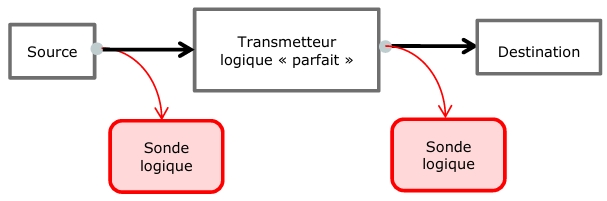
\includegraphics[width=0.7\linewidth]{figures/chaien_iteration_3.png}
    \caption{Modélisation de la chaîne de transmission à l’étape 1. Source : sujet.}
    \label{fig:fig1}
\end{figure}

\section{Résultats attendus}
Le résultat attendu est une transmission parfaite du signal (aucune modification du message).
En effet, l'information transmise durant cette première itération reste une suite binaire et n'est jamais convertie en signal analogique. Ainsi, aucune erreur et aucun bruit ne sont censés perturber la transmission.

\pagebreak

\section{Résultats observés}
Les résultats montrent que tout fonctionne comme attendu, on peut envoyer des messages choisis et aléatoires, et on constate que le \gls{teb} reste à 0 (voir figure \ref{fig:TestI1-2}).
\begin{figure}[H]
    \centering
    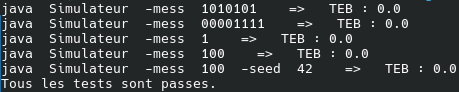
\includegraphics[width=0.8\linewidth]{figures/test_I1-1.png}
    \caption{Test automatisé pour l'itération 1. Source : capture d'écran du logiciel.}
    \label{fig:TestI1-2}
\end{figure}

On peut également effectuer un test supplémentaire en plaçant une sonde au niveau de la source et après le transmetteur. Ici encore, on observe que le graphique est le même, ce qui signifie que le message n'a pas été altéré lors de sa transmission (voir figure \ref{fig:TestI1-3}).

\begin{figure}[H]
    \centering
    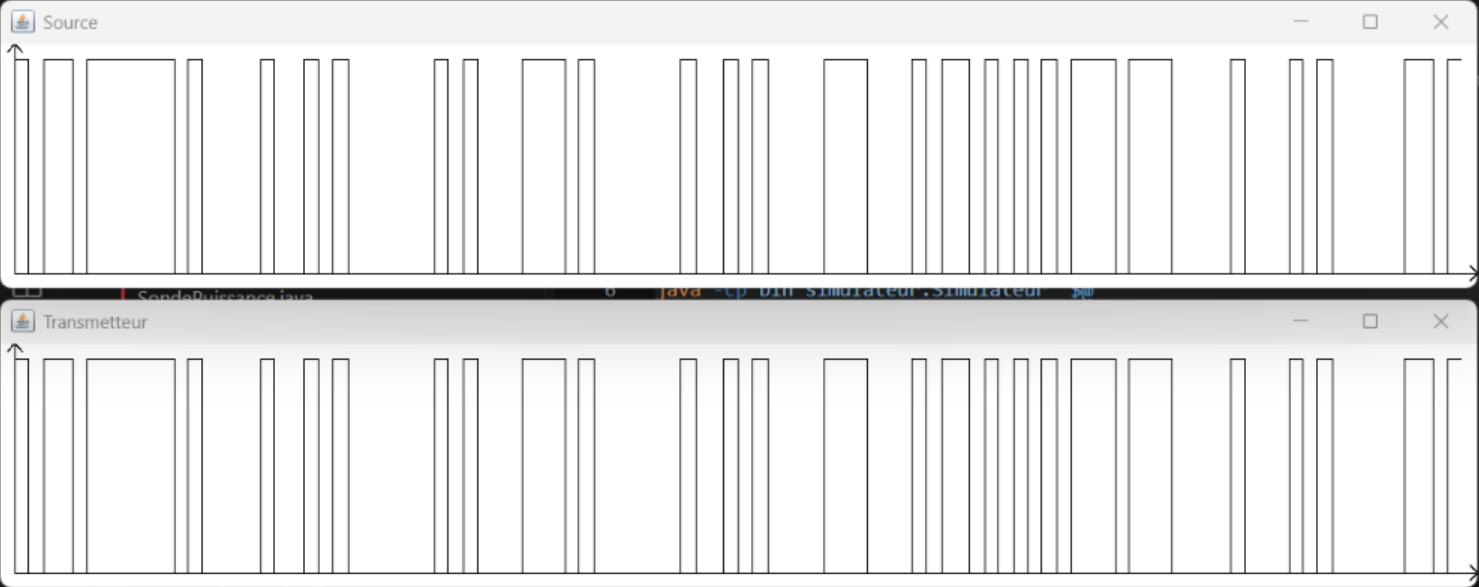
\includegraphics[width=0.8\linewidth]{figures/test_I1-2.png}
    \caption{Graphique représentant le message binaire à la source et après le transmetteur. Source : capture d'écran du logiciel.}
    \label{fig:TestI1-3}
\end{figure}

Pour observer de tels résultats, nous avons dû tester plusieurs cas d'utilisation du programme grâce aux paramètres du script bash "simulateur". Étant donné que nous n'avions pas encore codé de tests java, nous avons décidé de nous aider de l'intelligence artificielle Gemini pour terminer de prendre en main la méthode de lancement du simulateur et tester notre travail. Celle-ci a écrit des tests en bash qui nous ont permis de valider le bon fonctionnement de notre simulateur. Néanmoins, pour les itérations suivantes, notre enseignant de programmation nous a recommandé de plutôt utiliser des test Java comme enseigné en classe. Lors du travail sur l'itération 2, nous en avons donc profité pour écrire des tests Java pour les itérations 1 et 2. Ces derniers passent et valident le code de l'itération 1.

\section{Conclusion}
Le résultat obtenu est une transmission parfaite du signal, comme attendu. Celui-ci a, en effet, conservé sa forme binaire tout au long de la transmission et n'a pas été altéré.
Du point de vue de la transmission, l’étape 1 est réussie.

\chapter{Itération n°2 : Transmission analogique non bruitée}
\thispagestyle{main}

\section{Rappel des objectifs de l'itération}
Dans la première itération, nous avons simulé la transmission d'une information conservant sa forme binaire tout au long de sa transmission. Il en a résulté la réception de l'information sans aucune erreur binaire.

La seconde itération consiste à simuler une transmission élémentaire via un transmetteur analogique \og{}parfait\fg{}. Autrement dit, l'information ne restera pas sous forme binaire logique (simple suite de 0 et de 1) tout au long de la transmission, mais sera convertie sous forme d'un signal analogique simulé pour une partie de la transmission. Le transmetteur étant parfait, nous n'intégrons pas de bruit pour cette itération. Il s'agit alors d'une mise en application physique d'une transmission d'information en analogique en prenant en compte les défauts de ce mode de transmission sans bruit. La chaîne de transmission est modélisée dans la figure \ref{fig:fig21}.

\begin{figure}[H]
    \centering
    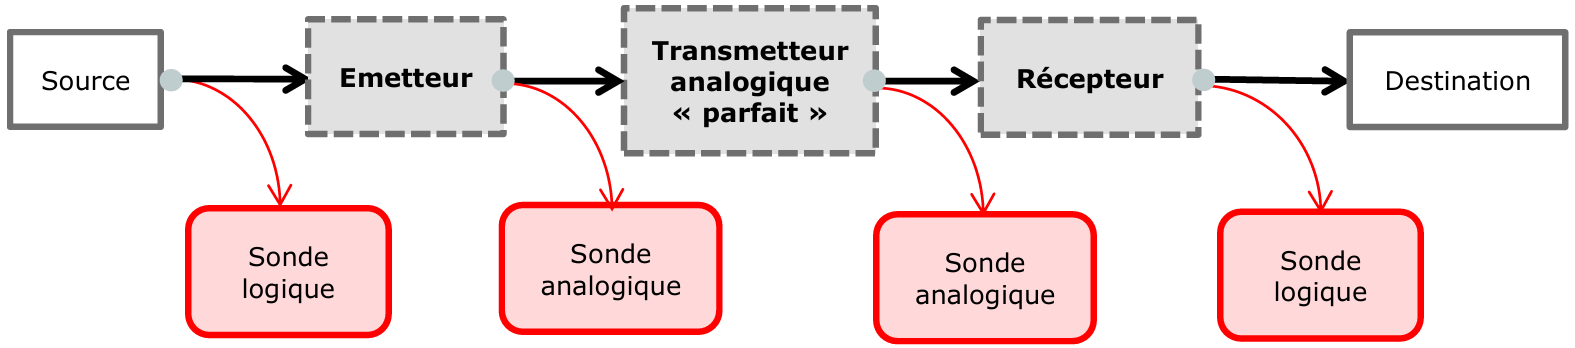
\includegraphics[width=0.9\linewidth]{figures/chaine_iteration_2.png}
    \caption{Modélisation de la chaîne de transmission à l’étape 2. Source : sujet.}
    \label{fig:fig21}
\end{figure}

C'est également au début de cette itération que le projet est fusionné avec celui d'un autre groupe. Cela introduit un travail supplémentaire en début d'itération afin d'étudier quels éléments sont à garder de quel projet. Après étude des deux projets à fusionner, il a été décidé de garder le code d'un seul des deux projets (cela permet d'éviter les fusions de code qui peuvent s'avérer fastidieuses) et de garder la partie rapport de l'autre projet. Enfin, à la suite du bureau d'étude sur l'organisation, nous avons établi une manière de travailler efficacement à 4 en gardant le meilleur des méthodes de travail établies par chacun des deux groupes. Ces méthodes de travail seront également mises à l'épreuve lors de cette 2e itération et seront éventuellement retravaillées si besoin à la fin de celle-ci.

Pour cette itération, le signal peut être codé avec trois formes d'ondes différentes :
\begin{itemize}
  \item \gls{nrz}
  \item \gls{nrzt}
  \item \gls{rz} (voir figure \ref{fig:fig22})
\end{itemize}

\begin{figure}[H]
    \centering
    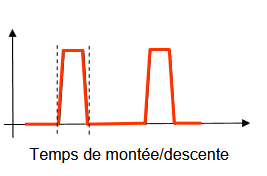
\includegraphics[width=0.5\linewidth]{figures/NRZ_analogique_TP2.png}
    \caption{Exemple d'un signal analogique \gls{rz}. Source : sujet.}
    \label{fig:fig22}
\end{figure}

\section{Résultats attendus}
En l'absence de bruit et de distorsion sur le canal de transmission parfait :
\begin{itemize}
    \item \textbf{Intégrité du signal analogique :} Le signal présent à l'entrée du récepteur doit être strictement identique, échantillon par échantillon, au signal émis en sortie de l'émetteur ($s_{recu}(t) = s_{emis}(t)$).
    \item \textbf{Taux d'Erreur Binaire (\gls{teb}) :} La séquence binaire reçue par la destination devant être rigoureusement identique à la séquence émise par la source, le \gls{teb} théorique attendu est strictement nul :
    \[
        \text{TEB} = 0{,}0
    \]
    \item \textbf{Validation temporelle :} La forme d'onde visualisée sur les sondes analogiques doit refléter fidèlement le codage choisi (paliers horizontaux pour le \gls{nrz}, transitions linéaires/trapézoïdales pour le \gls{nrzt}, retours à zéro sur les deuxièmes tiers de symbole pour le \gls{rz}).
\end{itemize}


\section{Résultats observés}

Conformément aux recommandations de l'enseignant de programmation, nous avons développé et utilisé des tests Java pour cette seconde itération. Ces tests nous permettent de valider le bon fonctionnement de notre code et sa non-régression tout au cours du développement. 

Par exemple, si nous nous attendons à ce qu'une transmission en particulier ait un \gls{teb} égal à 0, nous l'écrivons dans le test associé. Si finalement le \gls{teb} est égal à 0.5, alors une erreur est levée et nous savons immédiatement que la transmission n'a pas été simulée comme elle aurait dû l'être.

En parallèle, nous lançons manuellement des tests de transmissions pour vérifier de manière plus visuelle la bonne transmission ou non du message. Cela nous permet d'observer les signaux captés par les sondes et de les comparer entre eux. Ainsi, nous pouvons travailler notre code jusqu'à ce qu'il permette de simuler les transmissions de la manière attendue. L'objectif de ces tests manuels est aussi de vous présenter les résultats suivants.

\bigskip

Observons la figure \ref{fig:resultats2.3} qui illustre notre chaîne de transmission simulée pour un message via un signal \gls{nrzt}.

\begin{figure}[H]
    \centering
    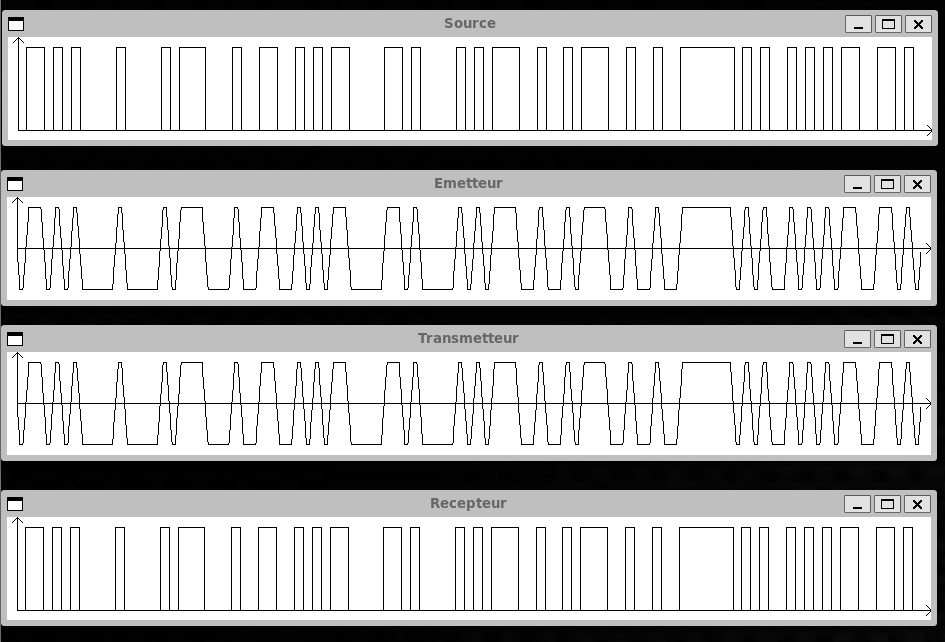
\includegraphics[width=0.9\linewidth]{figures/TP2_resultats.png}
    \caption{Chaîne de transmission d'un message \gls{nrzt}. Source : capture d'écran du logiciel.}
    \label{fig:resultats2.3}
\end{figure}

On peut remarquer que les résultats sont exactement ceux attendus, avec le message de la source qui est le même que celui du récepteur. Aussi, l'émetteur émet bien un message analogique de type \gls{nrzt} et le transmetteur transmet également le message sous la même forme, puis le récepteur remet en forme le message. Le \gls{teb} est donc égal à 0, ce qui est aussi attendu. 

Nous avons également simulé la transmission de différents messages avec les formes \gls{nrz} et \gls{rz}. Celles-ci se sont également parfaitement déroulées, avec un \gls{teb} égal à 0.

\section{Utilisation de l'IA}
Pour réaliser les itérations de ce projet, nous nous sommes aidés de différents \gls{llm}, mais principalement de Gemini. Le choix de ce modèle repose principalement sur sa polyvalence et son offre étudiante gratuite. Claude est une alternative similaire que nous utilisations également, mais qui possède des limites d'utilisation plus strictes. Nous utilisons également Mistral Vibe quand nous souhaitons une meilleure protection des données que nous voulons faire traiter par l'IA.

Un bilan plus détaillé de l'utilisation des IA dans la phase de développement apparaît, prompts compris, dans le fichier \verb|ai_prompts.md| de notre livrable.

Tout d'abord, Gemini nous a été utile pour rédiger ce rapport. En effet, nous ne sommes pas tous familiers avec LaTeX, le langage que nous utilisons pour écrire ce document. Pour ne pas avoir besoin de chercher dans la documentation, nous avons notamment demandé à Gemini comment insérer une liste à points, des acronymes, des sauts de page ou des espaces entre les paragraphes. Grâce à l'IA, nous avons pu mémoriser ces mots-clés afin de produire un rapport de qualité.

Ensuite, Gemini a aussi été utile pour résoudre des problèmes spécifiques à notre environnement de développement : VSCode. Il nous a notamment permis de réactiver une fonctionnalité permettant de fusionner nos codes en cas de conflits détectés par le logiciel Git que nous utilisons. Gemini nous a aussi permis de trouver d'où venaient certains problèmes de compilation du code, et de corriger nos scripts en conséquence. Ainsi, nous sommes montés en compétences sur VSCode et Java.

De plus, Gemini nous a aidé à rendre compatibles avec JUnit et Emma les tests Java que nous avions développés. Nous avons fait cela à la suite de la recommandation de l'enseignant de programmation. Notre programme est donc maintenant plus facile à tester, ce qui limite le nombre d'erreurs de nos simulations. Gemini a aussi généré des tests utilisant de language Bash. Ces tests bonus nous permettent de tester à la fois le fonctionnement de nos scripts Bash et Java. Cela nous permet de nous assurer de la compatibilité de notre code avec notre environnement de développement et de livraison.

Enfin, nous avons demandé à Mistral Vibe d'analyser notre code et de vérifier s'il implémente correctement et intégralement les exigences de l'étape 2. Étant donné que cette demande implique de fournir tout notre code à l'IA, nous avons utilisé Mistral Vibe pour une meilleure protection des données.

\pagebreak

\section{Conclusion}

Le résultat obtenu est une transmission parfaite du signal, comme attendu. 

Contrairement à l'itération 1, le message n'est pas resté sous forme binaire tout au long de la transmission. Il a pris la forme de signaux, de types différents (\gls{nrz}, \gls{nrzt}, \gls{rz}) selon la méthode de transmission choisie. Dans ces trois situations, le message n'a pas été altéré car le message reçu est identique au signal émis. En effet, nous n'avons ajouté ni bruit, ni autre type d'altération du signal. Cela nous a permis de parfaitement réceptionner le signal avec un récepteur basique. 

D’un point de vue transmission, l’étape 2 est donc réussie.

\chapter{Itération n°3 : Transmission analogique bruitée (bruit gaussien)}

\section{Rappel des objectifs de l'itération}

Dans cette troisième itération, le but est d'introduire un bruit gaussien au signal. Ce bruit ajouté permettra de revoir les notions de bruits gaussien, du \gls{snr} et du \gls{teb}. La chaîne de transmission pour cette troisième itération est modélisée dans la figure \ref{fig:fig31}.

On utilisera l'équation suivante pour définir le SNR par bit en dB :

\begin{equation*}
\left(\frac{Eb}{N_0}\right)_{\mathrm{dB}} = 10 \log_{10} \left(\frac{P_s \times N}{2\sigma_b^2}\right)
\end{equation*}


\noindent{Détail des termes :}
\begin{itemize}
    \item $E_b$ : Énergie par bit d'information
    \item $N_0$ : Densité spectrale de puissance du bruit
    \item $P_s$ : Puissance du signal reçu
    \item $N$ : Facteur d'étalement ou nombre d'échantillons
    \item $\sigma_b^2$ : Variance de la composante de bruit
\end{itemize}

\begin{figure}[H]
    \centering
    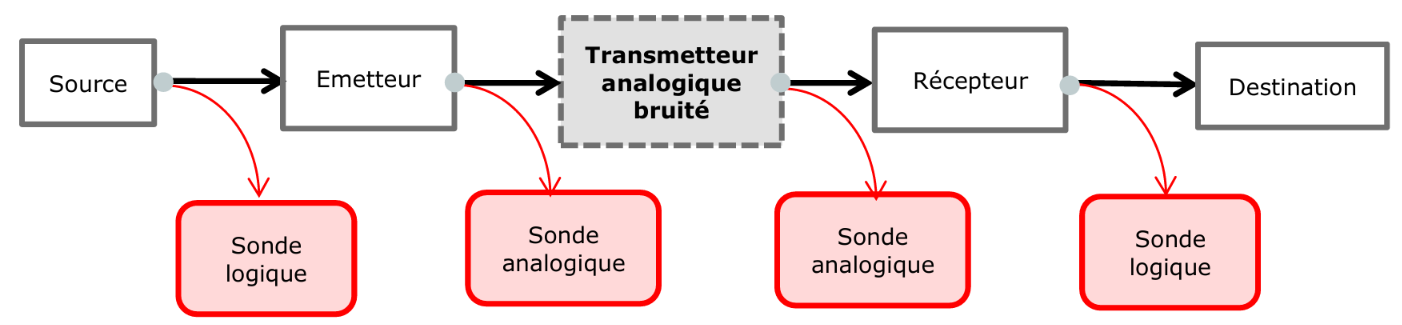
\includegraphics[width=0.9\linewidth]{figures/chaine_iteration_3.png}
    \caption{Modélisation de la chaîne de transmission à l’étape 3. Source : sujet}
    \label{fig:fig31}
\end{figure}

\pagebreak

\section{Résultats attendus}

Pour cette itération, nous nous attendons plusieurs résultats. 

\subsection{Bruit gaussien}

Le premier résultat attendu est que le bruit soit gaussien. Pour s'y prendre, nous afficherons un histogramme du bruit. Nous nous attendons à voir deux schémas ressemblant à ceux représentés dans la figure \ref{fig:fig32}.

\begin{figure}[H]
    \centering
    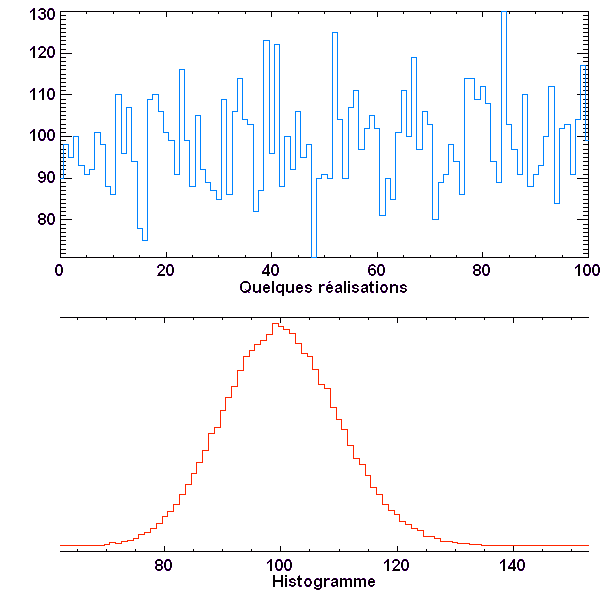
\includegraphics[width=0.5\linewidth]{figures/histogramme_gausse.png}
    \caption{Représentation d'une variable aléatoire et de son histogramme. Source : \href{https://media4.obspm.fr/public/ressources_lu/pages_analyser/impression.html}{Astrophysique sur Mesure}.}
    \label{fig:fig32}
\end{figure}

\subsection{Taux d'erreur binaire}

Après avoir vérifié que le bruit soit bien gaussien, nous pouvons faire un schéma du rapport entre l'énergie d'un Bit $E_b$ par la densité spectrale de bruit $N_0$ en fonction de l'erreur binaire. La figure \ref{fig:fig33} représente une allure générale de l'évolution du \gls{teb} en fonction du \gls{snr} par bit, pour différentes modulations.

\begin{figure}[H]
    \centering
    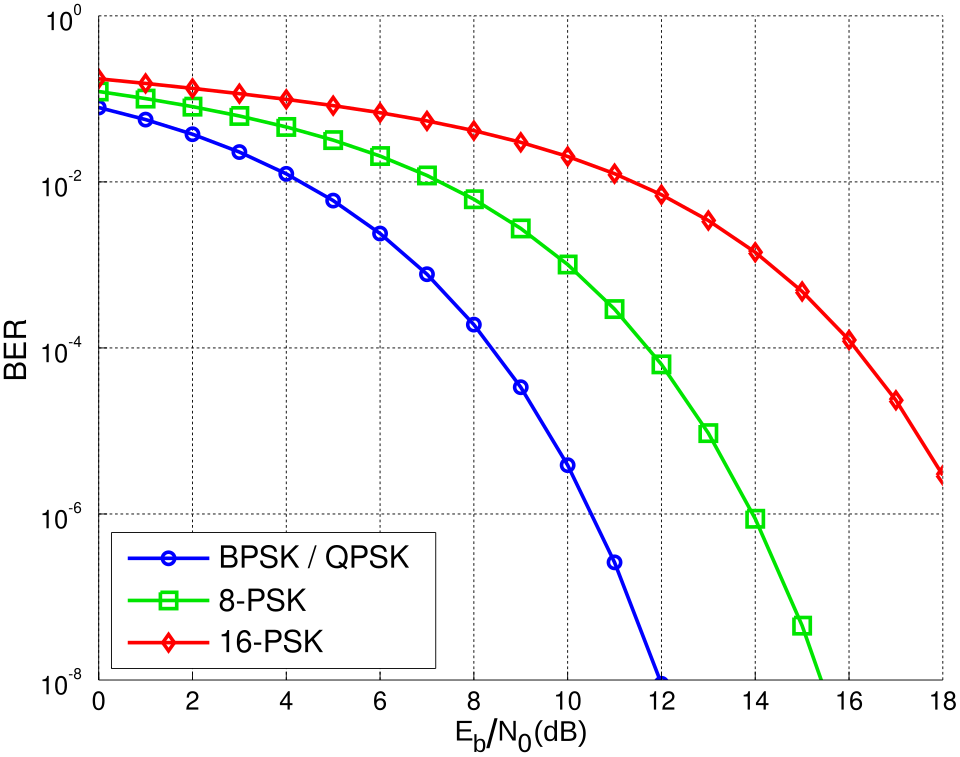
\includegraphics[width=0.4\linewidth]{figures/energiebit_rapportDSP.png}
    \caption{Graphique du \gls{teb} par rapport au $E_b/N_0$ en fonction de la modulation. Source : \href{https://en.wikipedia.org/wiki/Eb/N0}{Wikipédia}.}
    \label{fig:fig33}
\end{figure}

Dans le cadre de notre projet, nous nous attendons à ce que notre TEB par rapport à notre \gls{snr} par bit ait une allure similaire à la figure \ref{fig:fig33}. Nous générerons pour cela notre propre courbe.

\bigskip

Pour cela, nous avons codé le récepteur de manière à ce qu'il retrouve autant que possible le signal original. Pour ce faire, le récepteur moyennera les échantillons de chaque bit pour réduire l'impact du bruit aléatoire, puis décide du bit en comparant cette moyenne à un seuil fixé entre les amplitudes min et max. Pour l'instant, avec un bruit blanc gaussien centré en 0, on sait que sur le temps d'un bit la moyenne du bruit sera de 0. Ainsi, la valeur du signal ne changera pas tant que le \gls{snr} restera faible et que le bruit ne sera pas trop important pour induire des erreurs au niveau du récepteur. 

Le récepteur reconstitue chaque bit en 3 étapes :

\begin{enumerate}
    \item \textbf{Moyenne} des échantillons du bit :
    \begin{itemize}
        \item NRZ : tous les échantillons
        \item RZ/NRZT : tiers central (évite les transitions)
    \end{itemize}

    \item \textbf{Seuil} : $S = \frac{A_{min} + A_{max}}{2}$

    \item \textbf{Décision} :
    \[
    \text{bit} =
    \begin{cases}
        1 & \text{si moyenne} > S \\
        0 & \text{sinon}
    \end{cases}
    \]
\end{enumerate}

\sout{Après avoir codé nous avons placé la sonde sur le transmetteur et nous retrouvons bien le signal bruité, voir figure \ref{fig:fig34}.}

\begin{figure}[H]
    \centering
    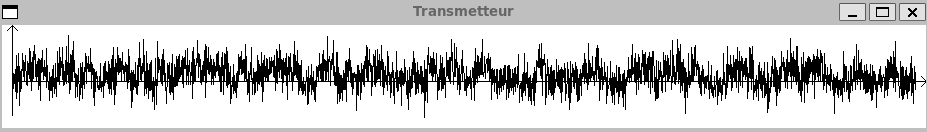
\includegraphics[width=0.8\linewidth]{figures/transmetteur_bruite.png}
    \caption{Signal du transmetteur. Source : capture d'écran du logiciel.}
    \label{fig:fig34}
\end{figure}

\subsection{Puissance du signal et écart-type du bruit}

Après avoir vérifier que nous pouvons injecter du bruit dans le transmetteur nous allons vérifier si les valeurs théoriques coïncides bien avec les valeurs trouvées avec le code. 

Puissance du signal :

$$P_s = \lim_{K \to +\infty} \frac{1}{K}\sum_{n=1}^{K} s^2(n)$$

\gls{snr} par bit :

$$\left(\frac{E_b}{N_0}\right){\text{dB}} = 10\log{}\left(\frac{P_s \times N}{2\sigma_b^2}\right)$$

d'où l'écart-type du bruit :

$$\sigma_b = \sqrt{\frac{P_s \times N}{2 \times 10^{(E_b/N_0)_{\text{dB}}/10}}}$$

Pour notre test la classe TestTP3.java envoie au transmetteur bruité un signal test de 100 échantillons : 50 à la valeur 1,0 puis 50 à la valeur 0,0, avec $snrpb$ = 10 dB et $N$ = 30. Le code effectue ces étapes suivantes :

\vspace{0.5cm}

Étape 1 — Puissance du signal :

$P_s = \frac{1}{100}\sum_{n=1}^{100} s^2(n) = \frac{50 \times 1^2 + 50 \times 0^2}{100} = 0{,}5$

\vspace{0.5cm}

Étape 2 — Conversion du \gls{snr} en linéaire :

$10^{(snrpb)_{\text{dB}}/10} = 10^{10/10} = 10$

\vspace{0.5cm}

On sait que : 

\begin{align*}
\left(\frac{E_b}{N_0}\right)_{\text{dB}}
    &= 10\,\log_{10}\left(\frac{P_s \times N}{2\sigma_b^2}\right)\\[4pt]
\Longleftrightarrow \quad
10^{(E_b/N_0)_{\text{dB}}/10}
    &= \frac{P_s \times N}{2\sigma_b^2}\\[4pt]
\Longleftrightarrow \quad
\sigma_b
    &= \sqrt{\frac{P_s \times N}{2 \times 10^{(E_b/N_0)_{\text{dB}}/10}}}
\end{align*}

Étape 3 — Écart-type du bruit :

$\sigma_b = \sqrt{\frac{P_s \times N}{2 \times 10}} = \sqrt{\frac{0{,}5 \times 30}{20}} = \sqrt{0{,}75} \approx 0{,}866$

\vspace{0.5cm}

On obtient donc les résultats suivants, que nous vérifierons dans la partie Résultats observés :
\begin{itemize}
    \item Puissance du signal Ps = 0,5
    \item Ecart-type : $sigma_b \approx 0,866$
\end{itemize}

\section{Résultats observés}

\subsection{Bruit gaussien}
Tout d'abord, vérifions si le bruit que nous avons inclus dans la chaine de transmission est bien gaussien.

Pour cela, isolons le bruit et mettons le sur un histogramme, comme montré sur la figure \ref{fig:fig35}.

Pour ce test, nous avons mis en place un bruit avec 50 000 échantillons pour essayer d'avoir une forme gaussienne, car l'aléatoire sur seulement quelques échantillons peut ne pas être suffisement représentatif pour former une gaussienne. 

\begin{figure}[H]
    \centering
    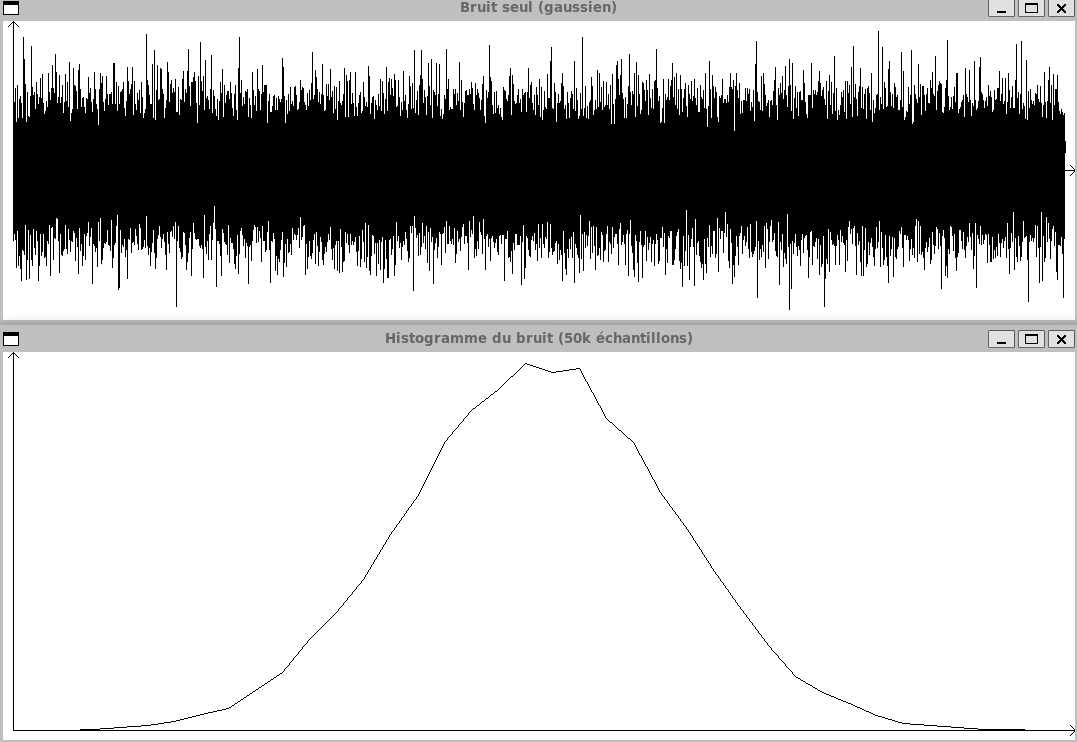
\includegraphics[width=0.75\linewidth]{figures/bruit_histogram.png}
    \caption{Histogramme bruit gaussien}
    \label{fig:fig35}
\end{figure}

Nous obtenons sur la figure \ref{fig:fig35} une gaussienne centré sur 0 avec une forme en cloche. 

\subsection{Taux d'erreur binaire}

\sout{Après avoir validé les tests avec des signaux théorique nous allons simuler à partir du message partant de l'émetteur avec un signal \gls{nrzt}, allant de +5 à -5, un \gls{snr} de -8 dB et un message de 100 bits nous obtenons la chaîne de transmission représentée en figure \ref{fig:fig36}.}

\begin{figure}[H]
    \centering
    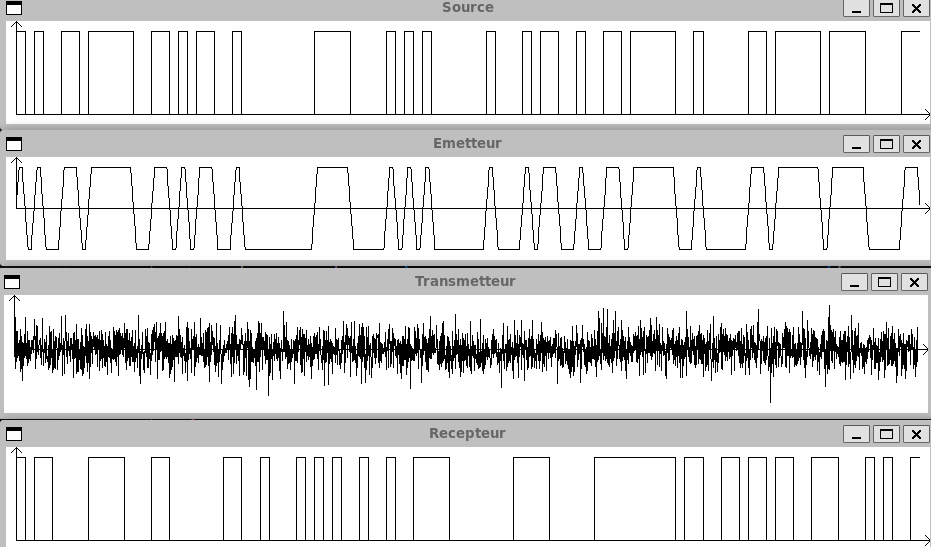
\includegraphics[width=1\linewidth]{figures/resultat_tp4_teb.png}
    \caption{Chaîne de transmission bruité gaussienne}
    \label{fig:fig36}
\end{figure}

\sout{A partir des résultats de cette chaîne de transmission nous obtenons un taux d'erreur binaire de 0.36, ce qui est normal du fait que le bruit est très important, et il est possible de le constater en regardant la différence entre le message "Source" et le message "Récepteur" les 2 sont différents.}

Notre enseignant nous a fait remarquer qu’une seule valeur de TEB n’a pas réellement de sens pour le simulateur. L’idée est donc de tracer le TEB en fonction du rapport $E_b/N_0$, exprimé en dB, qui correspond au rapport entre l’énergie par bit et la densité spectrale de puissance du bruit.

Cela nous permet, à partir de la théorie, d’estimer le TEB et de comparer ces résultats avec ceux obtenus à l’aide de notre simulateur.

Dans notre expérience, la simulation est réalisée avec un message de 100 000 bits, en faisant varier progressivement le rapport $E_b/N_0$. Une fonction nommée \texttt{gen-courbe.java} a été créée afin de générer un fichier CSV contenant, pour chaque type de signal, les valeurs du TEB en fonction du rapport $E_b/N_0$.

Enfin, un script Python est utilisé pour tracer les courbes obtenues (voir figure 3.7) et permettre leur comparaison avec les résultats théoriques.

Le récepteur moyenne les échantillons d'une fenêtre d'observation $I$, puis
compare cette moyenne $z$ à un seuil. La probabilité d'erreur ne dépend que de
deux grandeurs : la distance $d$ entre les deux valeurs moyennes possibles de
$z$, et l'écart-type du bruit sur cette moyenne :

\begin{equation*}
P_e = Q\!\left(\frac{d}{2\sigma_z}\right),
\qquad
Q(x) = \frac{1}{2}\,\mathrm{erfc}\!\left(\frac{x}{\sqrt{2}}\right),
\qquad
\sigma_z^{\,2} = \frac{\sigma_b^{\,2}}{|I|}
\end{equation*}

En injectant l'expression de $\sigma_b$ établie plus haut et en notant
$\gamma = E_b/N_0$ le rapport signal sur bruit par bit en linéaire, on obtient
pour chacune des trois formes d'onde :

\begin{align*}
P_e^{\gls{nrz}}  &= Q\!\left(\sqrt{2\gamma}\right) \\[6pt]
P_e^{\gls{rz}}   &= Q\!\left(\sqrt{\gamma}\right) \\[6pt]
P_e^{\gls{nrzt}} &= Q\!\left(\sqrt{\tfrac{6}{7}\,\gamma}\right)
\end{align*}

\begin{table}[H]
\centering
\begin{tabular}{lccc}
\hline
Forme d'onde & Niveaux & $P_e$ & Écart au \gls{nrz} \\
\hline
\gls{nrz}  & $-A$ et $+A$ & $Q\!\left(\sqrt{2\gamma}\right)$     & $0$ dB \\
\gls{rz}   & $0$ et $A$   & $Q\!\left(\sqrt{\gamma}\right)$      & $-3{,}0$ dB \\
\gls{nrzt} & $-A$ et $+A$ & $Q\!\left(\sqrt{6\gamma/7}\right)$   & $-3{,}7$ dB \\
\hline
\end{tabular}
\caption{\gls{teb} théorique des trois formes d'onde, avec $\gamma = E_b/N_0$.}
\label{tab:teb-theorique}
\end{table}

\paragraph{Interprétation.}
La fonction $Q$ donne la probabilité que le bruit dépasse la moitié de l'écart
entre les deux niveaux. Elle décroît très vite : plus son argument est grand,
plus la transmission est fiable.

\begin{itemize}
    \item Le \gls{nrz} utilise deux niveaux opposés, $-A$ et $+A$. L'écart
          entre un $0$ et un $1$ est donc deux fois plus grand qu'avec des
          niveaux $0$ et $A$, d'où le facteur $2$ sous la racine. C'est la
          forme d'onde la plus robuste.
    \item Le \gls{rz} n'utilise que les niveaux $0$ et $A$, ce qui divise
          l'écart par deux et coûte $3$ dB. Cette perte provient du choix des
          niveaux et non du retour à zéro : un \gls{nrz} de niveaux $0$ et $A$
          donnerait exactement le même résultat.
    \item Le \gls{nrzt} possède les mêmes niveaux que le \gls{nrz}, mais notre
          récepteur n'observe que le plateau central et ignore l'énergie
          contenue dans les rampes. Ce gaspillage coûte $3{,}7$ dB. Un filtre
          adapté à la forme trapézoïdale, pondérant chaque échantillon par la
          valeur de l'impulsion, permettrait de retrouver la performance du
          \gls{nrz}.
\end{itemize}

\paragraph{Conditions de validité des mesures.}
L'estimation expérimentale du \gls{teb} nécessite d'observer un nombre suffisant d'erreurs. C'est la raison pour laquelle nous avons fait la simulation de la figure 3.7 avec 100 000 échantillons.


\begin{figure}[H]
    \centering
    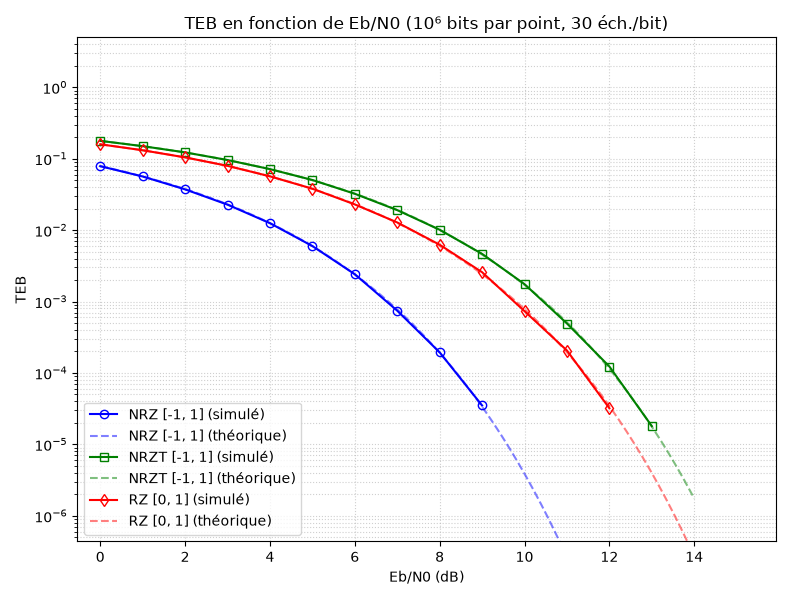
\includegraphics[width=0.5\linewidth]{Figure_1.png}
    \caption{TEB en fonction de Eb/N0}
    \label{fig:placeholder}
\end{figure}

La figure 3.7 nous montre des TEB cohérents, et une allure similaire à la figure 3.3.

\subsection{Puissance du signal et écart-type du bruit}

TestTP3 vérifie précisément que la puissance du signal mesurée par le code est bien Ps = 0,5 et que l'écart-type calculé est bien $sigma_b \approx 0,866$. Le calcul théorique coïncide avec notre chaine de transmission simulée.

\section{Utilisation de l'IA}
Intéressons-nous à différents usages que nous avons fait de l'IA pour cette itération. Nous nous sommes aidé de différents \gls{llm}. La justification de leurs utilisation est développée au chapitre 2.4 Utilisation de l'IA.
Un bilan plus détaillé de l'utilisation des IA dans la phase de développement apparaît, prompts compris, dans le fichier \verb|ai_prompts.md| de notre livrable.

Gemini nous a principalement été utile pour résoudre des problèmes que nous avons rencontrés dans la structuration de notre projet Java. Nous l'avons notamment utilisé pour déterminer qu'il était pertinent de fusionner les classes TransmetteurAnalogiqueBruite.java et TransmetteurBruite.java en une seule. Il nous a aussi permis de comprendre qu'il était nécessaire d'exclure nos classes de test du package test, afin de permettre le bon fonctionnement des outils de test JUnit et Emma dans notre environnement VSCode, ainsi que pour écrire certains tests bonus avec le langage Bash.

Pour les détails des calculs en format LaTeX (format du rapport), nous avons utilisé Mistral. Ce dernier a  été utilisé pour nous assister dans les calcul. Par exemple, le calcul de puissance n'était pas clair et Mistral a pu nous éclaircir sur ce point. 

Gemini a aussi été utile pour corriger des fautes d'orthographe et de syntaxe du rapport.

Pour écrire le script Python qui affiche les courbes de TEB, nous avons utilisé Claude. Ce dernier a été très efficace pour générer rapidement des courbes lisibles à partir des données que nous avions exportées.

\section{Conclusion}

En conclusion, nous avons pu analyser et calibrer une chaîne de transmission bruitée gaussienne, en y intégrant les différents signaux, messages et puissance de bruit. Nous avons pu vérifier, par le calcul et par l'observation de l'histogramme, que le bruit généré suit bien une loi gaussienne centrée.

Les tests d'intégration confirment également le comportement attendu du système : à fort rapport signal sur bruit, le taux d'erreur binaire est nul, tandis qu'à faible rapport, le bruit domine et le \gls{teb} devient élevé, la décision du récepteur tendant vers du
hasard. La reproductibilité des simulations grâce à la semence
\texttt{-seed} a aussi été validée.

\chapter{Itération n°4 : Transmission analogique à trajets multiples et bruitée}

\section{Amélioration des livrables précédents}
Cette itération est l'occasion pour nous de prendre en compte les commentaires et suggestions des enseignants pour améliorer notre logiciel et notre rapport. Pour cette raison, nous avons mis à jour le code et les rapports des itérations 2 et 3 afin qu'ils correspondent mieux aux attentes globale du projet, tant sur le fond que sur la forme.

Pour les itérations 2 et 3, nous avons réécris les chapitres 2.4 Utilisation de l'IA et 3.5 Utilisation de l'IA. Nous avons également corrigé des fautes d'orthographe et de syntaxe et référencé les figures qui ne l'étaient pas.

De plus, pour l'itération 3, nous avons revu les chapitres 3.2 Résultats attendus et 3.3 Résultats observés pour les clarifier et corriger les erreurs de mesure que nous avons faites. Les paragraphes barrés sont d'anciens paragraphes que nous avons remplacés.

\section{Rappel des objectifs de l'itération}


Jusqu'à présent, le canal de transmission ne comportait qu'un seul
trajet : le signal arrivait au récepteur sous la forme $s(t)$,
éventuellement bruité par un bruit blanc gaussien centré $b(t)$. En réalité,
un signal émis se propage dans l'environnement et se réfléchit sur
des obstacles (bâtiments, sol, ionosphère\dots). Le récepteur capte
alors la superposition du signal direct et de plusieurs échos
atténués et retardés.

Pour cette quatrième itération, nous modélisons le cas de trajets multiples : un trajet direct et un second trajet retardé et atténué, avec le bruit gaussien déjà introduit à l'itération précédente. Le signal reçu s'écrit :

$$r(t) = s(t) + \alpha\, s(t - \tau) + b(t)$$

avec :
\begin{itemize}
    \item $s(t)$ : le signal émis (trajet direct) ;
    \item $\alpha\, s(t-\tau)$ : le second trajet, atténué par
          $\alpha \in [0,1]$ et retardé de $\tau$ ;
    \item $b(t)$ : bruit blanc gaussien centré, comme au TP3.
\end{itemize}

Ce phénomène entraîne un déséquilibre à la réception : le signal reçu
n'est plus une copie du signal émis, mais une superposition
décalée dans le temps, ce qui déforme la forme d'onde et complique
la décision du récepteur.

\subsection{Démarche de simulation}

Pour que le récepteur puisse compenser ces effets, il doit connaître
les caractéristiques du canal : l' ou les atténuations $\alpha$ et le/les retard(s)
$\tau$. Or, nous avons fait le choix de ne pas transmettre ces paramètres au récepteur, dans l'objectif de rester \og{}~réalistes~\fg{}. Nous allons
donc utiliser un \textbf{message connu} (ou en-tête) : en début de transmission, la source émet un
message connu à la fois de l'émetteur et du récepteur.

Le récepteur, connaissant le message théorique, compare le signal
reçu correspondant au signal attendu et peut ainsi \textbf{estimer}
les effets du canal : le/les retard(s) $\tau$ et l' ou les atténuations $\alpha$. Une fois ces paramètres estimés, le récepteur peut corriger le signal reçu sur toute la suite de la transmission.

En résumé, la chaîne de transmission devient :

\begin{center}
Source $\rightarrow$ Émetteur $\rightarrow$ Transmetteur (trajets
multiples + bruit) $\rightarrow$ Récepteur $\rightarrow$ Destination
\end{center}

\subsection{Résultats attendus}

Avec cette modélisation, nous attendons les résultats suivants :

\begin{itemize}
    \item \textbf{Sans compensation} : le second trajet déforme le
          signal, le récepteur moyenne un signal faussé par l'écho,
          et le TEB est plus élevé qu'au TP3 (à SNR égal).
    \item \textbf{Avec compensation} ($\alpha$ et $\tau$ estimés via
          le message d'entraînement) : le récepteur soustrait l'écho
          du signal reçu, et le TEB doit redescendre vers les valeurs
          du TP3.
    \item \textbf{Cas limites} : pour $\alpha = 0$, on retrouve
          exactement le canal du TP3 (un seul trajet) ; pour
          $\alpha = 1$ et $\tau$ petit, l'écho est aussi fort que le
          signal direct et la transmission est fortement perturbée.
\end{itemize}

Pour vérifier ces résultats nous ferons des tests :

\begin{itemize}
    \item \textbf{Effets de l'amplitude} : Nous essaierons de voir l'évolution du TEB en fonction de l'amplitude $\alpha$  du signal retardé.
    \item \textbf{Effets du temps du retard} : Comme pour le test de l'influence de l'amplitude nous verrons l'influence de la taille du retard $\tau$ sur le TEB. 
    \item \textbf{Effet conjugué} : nous étudierons l'effet de la
      combinaison de $\alpha$ et $\tau$ sur le TEB, et vérifierons
      les cas limites : $\alpha = 0$ (retrouver le canal du TP3) et
      $\alpha = 1$ avec $\tau$ faible (écho aussi fort que le
      signal direct).
\end{itemize}

\section{Limites de notre égalisateur}

Lors de nos tests, nous avons rapidement constaté que notre égalisateur présente plusieurs limites.

Une première limite concerne le nombre de trajets multiples pouvant être détectés. Celui-ci est limité à cinq trajets, conformément aux consignes du projet. Notre algorithme de sondage recherche donc au maximum cinq retards différents.

Une deuxième limite concerne les retards des trajets multiples. Dans notre implémentation, le retard est exprimé en nombre d'échantillons et noté $d_k$. Le retard temporel correspondant est donné par :

$$
\tau_k = d_k T_e = \frac{d_k}{F_e},
$$

où $T_e$ est la période d'échantillonnage et $F_e$ la fréquence d'échantillonnage.

Notre algorithme impose :

$$
d_k \geq N_{\mathrm{ech}},
$$

où $N_{\mathrm{ech}}$ est le nombre d'échantillons par symbole. Dans notre configuration, $N_{\mathrm{ech}}=30$ : les trajets présentant un retard inférieur à 30 échantillons ne sont donc pas recherchés. Cette limitation vient de la méthode d'estimation utilisée : pour les formes d'onde NRZ, RZ et NRZT, les symboles sont constitués de plateaux de plusieurs échantillons, ce qui rend difficile la distinction entre un très faible retard et l'autocorrélation propre du signal.

L'estimation de plusieurs trajets présente également certaines difficultés lorsque leurs retards sont proches. Par exemple, avec deux trajets de retards $d_1=30$ et $d_2=150$ échantillons et de même amplitude, notre algorithme peut privilégier le second trajet lors de la recherche successive des pics de corrélation. Le premier trajet peut alors être moins bien détecté ou moins bien estimé. Ce comportement ne dépend cependant pas uniquement de l'écart entre les deux retards : la quantité d'en-tête disponible pour effectuer la corrélation dépend également du retard absolu.

Cela peut être observé en comparant ce cas avec celui de deux trajets présentant les retards $d_1=90$ et $d_2=210$ échantillons. L'écart entre les deux trajets est identique :

$$
150-30 = 210-90 = 120\text{ échantillons}.
$$

Pourtant, dans nos essais, les deux trajets sont alors correctement détectés et corrigés. Cette différence s'explique notamment par la portion de l'en-tête disponible pour l'estimation et par les corrélations obtenues pour chaque retard candidat. Notre méthode de détection étant gloutonne, le choix d'un premier trajet influence également la recherche des suivants.

Enfin, une limite concerne les amplitudes des trajets multiples. Le canal estimé est modélisé par :

$$
y[n] = x[n] + \sum_{k=1}^{K} a_k x[n-d_k],
$$

où $x[n]$ représente le trajet direct, $a_k$ l'amplitude relative du $k$-ième trajet multiple et $d_k$ son retard en échantillons.

L'égalisation consiste ensuite à inverser causalement ce canal selon la récurrence :

$$
\hat{x}[n]
=
y[n]
-
\sum_{k=1}^{K} a_k \hat{x}[n-d_k].
$$

L'égaliseur correspond ainsi au filtre IIR :

$$
G(z)
=
\frac{1}
{1+\displaystyle\sum_{k=1}^{K}a_kz^{-d_k}}.
$$

Une condition suffisante simple permettant de garantir la stabilité de cette inversion est :

$$
\sum_{k=1}^{K}|a_k| < 1.
$$

Dans notre implémentation, nous avons choisi une marge de sécurité et imposé :

$$
\boxed{\sum_{k=1}^{K}|a_k| < 0{,}90}.
$$

Cette marge permet d'éviter de travailler trop près de la limite théorique, où de faibles erreurs d'estimation des amplitudes ou des retards peuvent entraîner une forte amplification des erreurs par le filtre IIR.

Il est important de préciser que les coefficients $a_k$ considérés dans cette condition sont les amplitudes relatives estimées par le récepteur à partir du signal reçu. Ils peuvent donc légèrement différer des amplitudes définies lors de la génération du canal, notamment en raison de l'estimation par corrélation, du bruit et des approximations liées à la détection des retards.

Ainsi, même lorsqu'un canal respecte les paramètres définis à l'émission, l'égalisation peut être désactivée si les coefficients estimés par le récepteur ne respectent pas la condition de stabilité retenue.

\section{Résultats observés}

\section{Utilisation de l'IA}
Intéressons-nous à différents usages que nous avons fait de l'IA pour cette itération. Nous nous sommes aidé de différents \gls{llm}. La justification de leurs utilisation est développée au chapitre 2.4 Utilisation de l'IA.
Un bilan plus détaillé de l'utilisation des IA dans la phase de développement apparaît, prompts compris, dans le fichier \verb|ai_prompts.md| de notre livrable.

\begin{itemize}
    \item En vue d'améliorer les performances de notre programme, nous avons utilisé un LLM Claude pour identifier la source de nos problèmes de performance qui allongeait de plusieurs dizaines de minutes la durée nécessaire pour tester notre programme. L'enseignant de programmation nous a ensuite confirmé que le problème venait de la fonction de calcul du TEB, comme l'avait identifié l'IA. Nous avons ensuite corrigé le problème à la main.
    \item Gemini a été utile pour corriger des fautes d'orthographe et de syntaxe du rapport. Cet usage est particulièrement utile après une première relecture pour corriger des erreurs sans perdre de temps.
    \item Un fois le code terminé, nous avons demandé à Gemini de lire notre code pour nous signaler s'il trouvait des fonctionnalités qu'on avait oublié de développer.
\end{itemize}

\section{Conclusion}

\chapter{Itération n°5 : Codage de canal}
\thispagestyle{main}

\section{Rappel des objectifs de l'itération}

Dans les itérations précédentes, nous avons mis en place une chaîne de transmission analogique capable de modéliser des formes d'onde variées (\gls{nrz}, \gls{rz}, \gls{nrzt}), d'injecter un bruit blanc gaussien centré et de simuler des trajets indirects multiples. Toutefois, en présence de bruit, la démodulation effectuée par le récepteur conduit inévitablement à des erreurs binaires dès lors que le niveau de bruit dépasse le seuil de décision.

L'objectif de cette cinquième et dernière étape est d'introduire un \textbf{codage de canal} afin de protéger le message binaire contre les perturbations du canal et d'améliorer la qualité de service en réduisant le \gls{teb}. 

Pour cela, nous insérons :
\begin{itemize}
    \item Un composant de \textbf{codage en émission} (\texttt{CodeurCanal}), placé juste après la source logique et avant le modulateur analogique (émetteur) ;
    \item Un composant de \textbf{décodage en réception} (\texttt{DecodeurCanal}), placé juste après le démodulateur (récepteur) et avant la destination finale.
\end{itemize}

Une nouvelle option de ligne de commande \texttt{-codeur} permet d'activer conjointement ces deux éléments. Par défaut, le codage de canal n'est pas utilisé afin de préserver la compatibilité ascendante avec les itérations précédentes.

La figure \ref{fig:chaine_it5} illustre l'organisation générale de la chaîne de transmission incluant le codage de canal.

\begin{figure}[H]
    \centering
    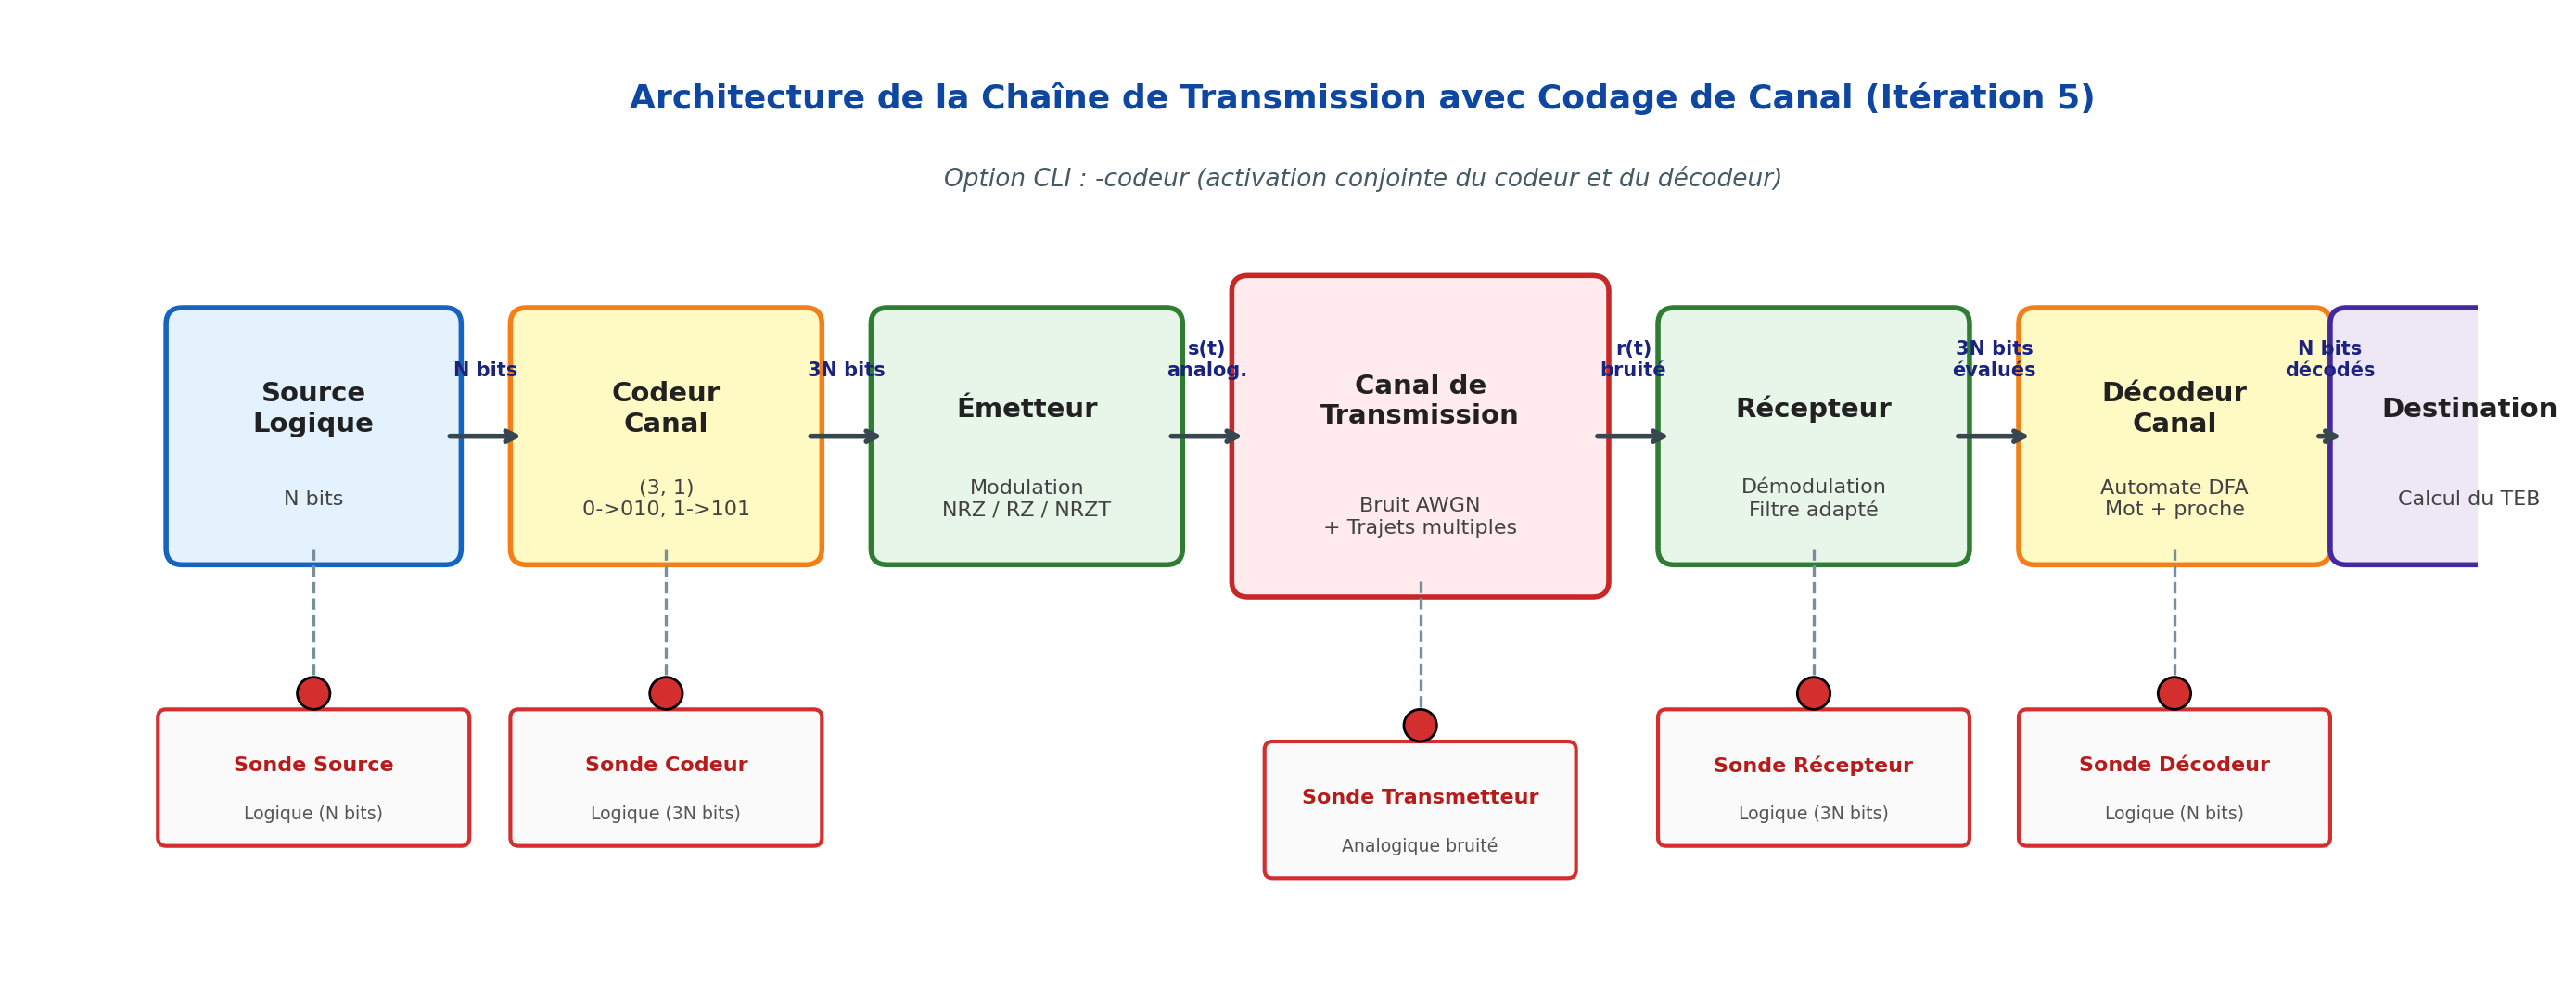
\includegraphics[width=0.95\linewidth]{figures/chaine_iteration_5.png}
    \caption{Modélisation de la chaîne de transmission à l'étape 5 avec codage de canal. \textit{(Figure à insérer : schéma synoptique Source $\to$ Codeur $\to$ Émetteur $\to$ Canal bruité $\to$ Récepteur $\to$ Décodeur $\to$ Destination)}}
    \label{fig:chaine_it5}
\end{figure}

\section{Principe et modélisation du codage retenu}

\subsection{Principe de l'encodeur}

Le dispositif d'émission transforme chaque bit d'information utile en une séquence de trois bits à transmettre sur le canal :
\begin{align*}
    0 &\longrightarrow 0\;1\;0 \\
    1 &\longrightarrow 1\;0\;1
\end{align*}

Ce code est un code en bloc binaire de paramètres $(n, k) = (3, 1)$ :
\begin{itemize}
    \item La longueur d'un mot d'information est $k = 1$ bit ;
    \item La longueur d'un mot de code transmis est $n = 3$ bits ;
    \item Le rendement de codage vaut $R = \frac{k}{n} = \frac{1}{3}$.
\end{itemize}

Ce codage présente deux avantages majeurs en ingénierie des télécommunications, que nous détaillons ci-après.

\subsection{Premier atout : facilitation de la synchronisation d'horloge}

Dans un système de transmission numérique réel, le récepteur doit synchroniser son horloge locale d'échantillonnage sur le rythme d'émission à l'aide d'une boucle à verrouillage de phase (PLL). Pour fonctionner correctement et éviter la dérive temporelle de l'horloge, ces circuits de récupération de rythme ont impérativement besoin de transitions régulières (fronts montants et descendants) dans le signal reçu. 

Or, une séquence prolongée de bits identiques (par exemple une longue suite de $0$ ou de $1$ en modulation \gls{nrz}) maintient le signal analogique à un niveau constant. En l'absence de transitions, l'horloge du récepteur glisse et la synchronisation peut être totalement perdue.

Le codage retenu résout élégamment ce problème :
\begin{itemize}
    \item Une suite continue de zéros ($0 \to 010$) produit le train binaire $010\,010\,010\dots$ : il y a au maximum deux zéros consécutifs (à la frontière entre deux blocs de trois bits).
    \item Une suite continue de uns ($1 \to 101$) produit le train binaire $101\,101\,101\dots$ : il y a au maximum deux uns consécutifs.
    \item Une alternance de bits ($0, 1 \to 010\,101$) ne présente jamais plus d'un bit identique consécutif ($0, 1, 0, 1, 0, 1$).
\end{itemize}

Ainsi, ce codage garantit mathématiquement qu'il n'y a \textbf{jamais plus de deux bits consécutifs de même valeur} dans le signal transmis, assurant une densité minimale de transitions très élevée sur le canal.

\subsection{Deuxième atout : détection et correction d'erreurs}

L'alphabet des mots de code émis est restreint à deux éléments parmi les huit triplets possibles de $\{0, 1\}^3$ :
\[
    \mathcal{C} = \left\{ C_0 = (0, 1, 0),\; C_1 = (1, 0, 1) \right\}
\]

La distance de Hamming $d(u, v)$ entre deux mots correspond au nombre de positions où les bits diffèrent. Ici, les trois positions diffèrent entre $C_0$ et $C_1$, ce qui donne une distance minimale :
\[
    d_{\min} = d(C_0, C_1) = 3
\]

En théorie des codes correcteurs, un code de distance minimale $d_{\min}$ permet de :
\begin{itemize}
    \item Détecter jusqu'à $e = d_{\min} - 1 = 2$ erreurs de transmission ;
    \item Corriger jusqu'à $t = \left\lfloor \frac{d_{\min} - 1}{2} \right\rfloor = \left\lfloor \frac{3 - 1}{2} \right\rfloor = 1$ erreur par triplet.
\end{itemize}

À la réception, le décodeur applique une règle de décision au sens du \textbf{maximum de vraisemblance} (décision dure) : si le triplet reçu n'est ni $010$ ni $101$, on lui associe le mot de code le plus proche au sens de la distance de Hamming. 

Comme $d(r, C_0) + d(r, C_1) = 3$ pour tout triplet reçu $r \in \{0, 1\}^3$, l'une des deux distances vaut toujours au plus 1 et l'autre au moins 2. Il n'existe donc aucune ambiguïté de décision. La table de décodage complète est résumée dans le tableau \ref{tab:decodage_triplets}.

\begin{table}[H]
\centering
\begin{tabular}{|c|c|c|c|c|c|}
\hline
\textbf{Triplet reçu} & $\mathbf{d(r, C_0)}$ & $\mathbf{d(r, C_1)}$ & \textbf{Bit décodé} & \textbf{Mot retenu} & \textbf{Bit corrigé (position)} \\
\hline
$0\;0\;0$ & $1$ & $2$ & \textbf{0} & $0\;1\;0$ & $2^{\text{ème}}$ bit (venait de $0\,\textbf{1}\,0$) \\
$0\;0\;1$ & $2$ & $1$ & \textbf{1} & $1\;0\;1$ & $1^{\text{er}}$ bit (venait de $\textbf{1}\,0\,1$) \\
$0\;1\;0$ & $0$ & $3$ & \textbf{0} & $0\;1\;0$ & Aucun (mot exact) \\
$0\;1\;1$ & $1$ & $2$ & \textbf{0} & $0\;1\;0$ & $3^{\text{ème}}$ bit (venait de $0\,1\,\textbf{0}$) \\
$1\;0\;0$ & $2$ & $1$ & \textbf{1} & $1\;0\;1$ & $3^{\text{ème}}$ bit (venait de $1\,0\,\textbf{1}$) \\
$1\;0\;1$ & $3$ & $0$ & \textbf{1} & $1\;0\;1$ & Aucun (mot exact) \\
$1\;1\;0$ & $1$ & $2$ & \textbf{0} & $0\;1\;0$ & $1^{\text{er}}$ bit (venait de $\textbf{0}\,1\,0$) \\
$1\;1\;1$ & $2$ & $1$ & \textbf{1} & $1\;0\;1$ & $2^{\text{ème}}$ bit (venait de $1\,\textbf{0}\,1$) \\
\hline
\end{tabular}
\caption{Table de décodage déterministe des 8 triplets et correction d'erreur associée.}
\label{tab:decodage_triplets}
\end{table}

\noindent \textbf{Remarque d'équivalence :} Sur le plan logique, décoder le triplet $(r_1, r_2, r_3)$ revient à inverser le bit central ($r_2' = \overline{r_2}$) puis à prendre la majorité des trois bits $(r_1, \overline{r_2}, r_3)$. En effet, en inversant le bit central lors de l'émission, $0 \to 000$ et $1 \to 111$ : ce code est donc isomorphe à un code à répétition d'ordre 3 avec inversion du deuxième symbole.

\subsection{Modélisation par un automate fini déterministe (DFA)}

Conformément aux objectifs pédagogiques de l'énoncé, nous avons formalisé le fonctionnement du récepteur à l'aide de la théorie des automates. 

Le décodeur est modélisé par un \textbf{automate fini déterministe synchrone avec émission} (transducteur fini déterministe) défini par le quintuplet $\mathcal{A} = (Q, \Sigma, \Gamma, \delta, q_0)$ où :
\begin{itemize}
    \item $Q = \{q_0, q_1, q_2\}$ est l'ensemble fini des états ;
    \item $\Sigma = \{0, 1\}$ est l'alphabet d'entrée (bits démodulés) ;
    \item $\Gamma = \{0, 1, \varepsilon\}$ est l'alphabet de sortie ($\varepsilon$ désignant l'absence d'émission) ;
    \item $q_0$ est l'état initial.
\end{itemize}

Les états possèdent une signification physique directe :
\begin{itemize}
    \item \textbf{État $q_0$ :} attente du premier bit d'un nouveau bloc de 3 bits. La réception de $b_1$ fait passer à l'état $q_1$ en mémorisant $b_1$ (sortie $\varepsilon$).
    \item \textbf{État $q_1$ :} attente du deuxième bit. La réception de $b_2$ fait passer à l'état $q_2$ en mémorisant $b_2$ (sortie $\varepsilon$).
    \item \textbf{État $q_2$ :} attente du troisième bit $b_3$. Dès réception de $b_3$, le triplet $(b_1, b_2, b_3)$ est complet : l'automate applique la fonction de décision $f(b_1, b_2, b_3)$ issue du tableau \ref{tab:decodage_triplets}, émet le bit reconstitué dans $\Gamma$ et retourne instantanément dans l'état $q_0$ pour le paquet suivant.
\end{itemize}

Ce formalisme illustre concrètement l'intérêt du \textbf{déterminisme} :
\begin{enumerate}
    \item \textbf{Absence totale d'ambiguïté :} pour tout état et tout bit reçu, la transition d'état et le bit émis sont définis de manière univoque.
    \item \textbf{Complexité minimale :} le décodage s'effectue en temps linéaire $O(N)$ par rapport au nombre de bits reçus, et avec un espace mémoire constant $O(1)$.
    \item \textbf{Robustesse logicielle :} aucun risque d'interblocage ou de boucle infinie, ce qui convient parfaitement aux contraintes temps réel des récepteurs de télécommunication.
\end{enumerate}

\section{Résultats attendus}

\subsection{Calcul théorique du Taux d'Erreur Binaire (TEB)}

Soit $p$ la probabilité d'erreur binaire sur le canal après démodulation (correspondant au \gls{teb} sans codage étudié aux itérations 2 et 3). En supposant que le bruit affecte de façon indépendante chaque échantillon et chaque symbole (canal binaire symétrique sans mémoire), la probabilité qu'un paquet de 3 bits comporte $k$ erreurs suit une loi binomiale $\mathcal{B}(3, p)$ :
\[
    P(k \text{ erreurs}) = \binom{3}{k} p^k (1 - p)^{3 - k}
\]

Le décodeur fonctionne de la manière suivante :
\begin{itemize}
    \item Si le paquet comporte $0$ erreur : le mot reçu est exact ($010$ ou $101$), le bit est correctement décodé.
    \item Si le paquet comporte $1$ erreur : le décodeur la détecte et la répare avec succès. Le bit décodé est correct.
    \item Si le paquet comporte $2$ erreurs : le mot reçu est plus proche de l'autre mot de code valide (à distance 1 au lieu de 2). Le décodeur commet une décision erronée.
    \item Si le paquet comporte $3$ erreurs : le mot reçu correspond exactement au mot de code opposé. Le décodeur prend la décision inverse.
\end{itemize}

Une erreur sur le bit d'information décodé survient donc si et seulement si le paquet de 3 bits subit 2 ou 3 erreurs sur le canal. La probabilité d'erreur après décodage $P_{e,\text{codé}}$ s'exprime ainsi :
\begin{align*}
    P_{e,\text{codé}} &= P(2 \text{ erreurs}) + P(3 \text{ erreurs}) \\
                      &= \binom{3}{2} p^2 (1 - p) + \binom{3}{3} p^3 \\
                      &= 3 p^2 (1 - p) + p^3 \\
                      &= 3 p^2 - 2 p^3
\end{align*}

Comparons $P_{e,\text{codé}}$ avec le \gls{teb} non codé $p$ :
\[
    P_{e,\text{codé}} < p \iff 3p^2 - 2p^3 < p \iff 3p - 2p^2 < 1 \iff (2p - 1)(p - 1) > 0
\]
Comme $p \le 1$, cette condition est vérifiée dès que :
\[
    p < 0{,}5
\]

Pour tout canal exploitable où le \gls{teb} brut est inférieur à $50\%$, le codage de canal diminue donc le taux d'erreur binaire. 

De plus, en régime asymptotique à fort rapport signal sur bruit ($p \ll 1$), le terme en $p^3$ devient négligeable devant $p^2$, ce qui donne :
\[
    P_{e,\text{codé}} \approx 3 p^2
\]

Cette relation quadratique montre que \textbf{la pente de la courbe de TEB en échelle semi-logarithmique est doublée}. Le tableau \ref{tab:theorie_teb_gain} illustre numériquement le gain théorique spectaculaire apporté par le codage.

\begin{table}[H]
\centering
\begin{tabular}{|c|c|c|}
\hline
\textbf{TEB brut canal ($p$)} & \textbf{TEB après décodage ($3p^2 - 2p^3$)} & \textbf{Facteur d'amélioration} \\
\hline
$0{,}10$ ($10\%$) & $0{,}028$ ($2{,}8\%$) & $\times 3{,}6$ \\
$0{,}05$ ($5\%$) & $0{,}00725$ ($0{,}73\%$) & $\times 6{,}9$ \\
$0{,}01$ ($1\%$) & $0{,}000298$ ($\approx 0{,}03\%$) & $\times 33{,}6$ \\
$10^{-3}$ ($0{,}1\%$) & $2{,}998 \times 10^{-6}$ & $\times 333$ \\
$10^{-4}$ & $3{,}0 \times 10^{-8}$ & $\times 3\,333$ \\
\hline
\end{tabular}
\caption{Évolution théorique du TEB sous canal bruité avec et sans codage de canal.}
\label{tab:theorie_teb_gain}
\end{table}

\subsection{Compromis entre redondance, bande passante et énergie}

En contrepartie de cette réduction du \gls{teb}, le codage de canal introduit un coût physique :
\begin{enumerate}
    \item \textbf{Efficacité spectrale et débit :} Le rendement étant $R = 1/3$, il faut transmettre 3 fois plus de symboles pour transporter la même quantité d'information utile. Pour une durée de transmission identique, le débit utile est divisé par 3, ou la bande passante nécessaire est multipliée par 3.
    \item \textbf{Considération énergétique :} Si la puissance d'émission moyenne est constante, l'énergie par symbole transmis $E_c$ est liée à l'énergie par bit d'information $E_b$ par la relation :
    \[
        E_c = R \cdot E_b = \frac{E_b}{3} \implies \left(\frac{E_c}{N_0}\right)_{\text{dB}} = \left(\frac{E_b}{N_0}\right)_{\text{dB}} - 10 \log_{10}(3) \approx \left(\frac{E_b}{N_0}\right)_{\text{dB}} - 4{,}77\text{ dB}
    \]
    Dans notre simulateur, le paramètre \texttt{-snrpb} règle le rapport signal sur bruit par symbole de canal traversant le milieu de propagation. À paramètre \texttt{-snrpb} fixé, le gain en TEB est immédiatement mesurable.
\end{enumerate}

\subsection{Mise en évidence de l'amélioration de synchronisation : analyse critique}

La question 3 du sujet de TP5 nous interroge directement : \textit{\og{}Votre simulateur permet-il de mettre en évidence l'amélioration de synchronisation émetteur/récepteur promise par le transducteur ? Justifiez votre réponse.\fg{}}

La réponse est \textbf{non}, notre simulateur ne permet pas de mettre en évidence cette amélioration.

\paragraph{Justification détaillée :}
Dans notre simulateur, la synchronisation temporelle est \textbf{idéale et supposée parfaite à l'avance} :
\begin{itemize}
    \item Le récepteur connaît exactement le nombre d'échantillons par bit $N_{\text{ech}}$ (passé en paramètre au constructeur).
    \item Le récepteur découpe le signal analogique en tranches de taille $N_{\text{ech}}$ rigoureusement synchronisées à partir de l'indice 0 (ou après compensation du retard du canal).
    \item Notre modèle n'implémente aucun des défauts physiques réels qui affectent les horloges : pas de dérive fréquentielle ($\Delta F_e = 0$), pas d'instabilité de phase (gigue temporelle ou \textit{jitter}), et pas de circuit physique d'extraction de rythme (boucle de Gardner, PLL).
\end{itemize}

Par conséquent, que la source émette une séquence alternée ou une série continue de 10\,000 zéros consécutifs, l'échantillonnage s'effectue exactement aux mêmes instants optimaux. L'avantage du codage garantissant au plus 2 bits identiques successifs est fondamental sur une liaison physique réelle, mais reste totalement transparent et invisible dans notre environnement de simulation numérique idéal.

\section{Résultats observés}

\subsection{Validation logicielle et tests unitaires}

Afin de garantir la robustesse du code développé et sa non-régression, nous avons enrichi la suite de tests automatisés avec la classe \texttt{TestTP5.java}, intégrée à \texttt{TestSimulateur} et à \texttt{TestProjetJUnit}. 

L'ensemble des 38 tests unitaires et d'intégration du TP5 a été validé avec succès (100\% de réussite) :
\begin{itemize}
    \item \textbf{CodeurCanal :} vérification de l'expansion $0 \to 010$ et $1 \to 101$, conformité sur des séquences longues, et vérification algorithmique que la propriété de non-dépassement de 2 bits consécutifs identiques est bien respectée sur des séries de 500 zéros et 500 uns.
    \item \textbf{DecodeurCanal :} validation unitaire exhaustive des 8 combinaisons de triplets du tableau \ref{tab:decodage_triplets}, validation de la détection du bit erroné et des compteurs statistiques.
    \item \textbf{Test de correction d'erreurs :} sur un message transmis avec injection artificielle d'une erreur binaire sur chaque mot de code, le décodeur a corrigé 100\% des erreurs et restitué le message d'origine avec un TEB de $0{,}0$.
    \item \textbf{Intégration Simulateur :} validation de la transmission parfaite (TEB = 0,0) en logique pure, en analogique \gls{nrz}, \gls{rz}, \gls{nrzt}, ainsi qu'en combinaison avec les trajets multiples et le sondage de canal (\texttt{-ti} et \texttt{-sondage}).
\end{itemize}

\subsection{Mesures expérimentales du TEB sous canal bruité}

Conformément à la convention adoptée au chapitre 3 pour la comparaison avec la courbe théorique $Q(\sqrt{2\gamma})$, nous avons conduit une campagne de simulations numériques en modulation \gls{nrz} antipodale $[-1\text{ V}, +1\text{ V}]$ (\texttt{-ampl -1.0 1.0}) avec $100\,000$ bits par point (\texttt{-mess 100000}) et une graine fixe (\texttt{-seed 100}) afin de comparer le TEB obtenu avec et sans l'option \texttt{-codeur}, pour différents rapports $E_b/N_0$.

Les résultats obtenus sont présentés dans le tableau \ref{tab:resultats_mesures_teb}.

\begin{table}[H]
\centering
\begin{tabular}{|c|c|c|c|}
\hline
\textbf{SNR ($E_b/N_0$ en dB)} & \textbf{TEB sans codage ($p$)} & \textbf{TEB mesuré avec \texttt{-codeur}} & \textbf{TEB théorique ($3p^2 - 2p^3$)} \\
\hline
$0\text{ dB}$ & $0{,}07856$ (théo. $0{,}07865$) & $0{,}01704$ & $0{,}01758$ \\
$1\text{ dB}$ & $0{,}05590$ (théo. $0{,}05629$) & $0{,}00864$ & $0{,}00915$ \\
$2\text{ dB}$ & $0{,}03743$ (théo. $0{,}03751$) & $0{,}00396$ & $0{,}00412$ \\
$3\text{ dB}$ & $0{,}02295$ (théo. $0{,}02288$) & $0{,}00165$ & $0{,}00154$ \\
$4\text{ dB}$ & $0{,}01253$ (théo. $0{,}01250$) & $0{,}00055$ ($5{,}5 \times 10^{-4}$) & $0{,}00047$ \\
$6\text{ dB}$ & $0{,}00247$ (théo. $0{,}00239$) & $0{,}00002$ ($2{,}0 \times 10^{-5}$) & $0{,}000017$ \\
\hline
\end{tabular}
\caption{Comparaison des TEB mesurés expérimentalement (NRZ $[-1, 1]$) et de la prédiction théorique.}
\label{tab:resultats_mesures_teb}
\end{table}

\paragraph{Commentaires sur les résultats :}
\begin{itemize}
    \item La concordance entre les valeurs mesurées avec l'option \texttt{-codeur} et la formule théorique $3p^2 - 2p^3$ (avec $p = Q(\sqrt{2\gamma})$) est remarquable : à $0\text{ dB}$, le TEB simulé est de $0{,}01704$ pour $0{,}01758$ théorique ; à $4\text{ dB}$, il vaut $0{,}00055$ pour $0{,}00047$ théorique (écart inférieur à $10^{-4}$).
    \item À fort SNR (dès 4 à 6 dB), l'efficacité du codeur est spectaculaire : à $4\text{ dB}$, le TEB est divisé par près de \textbf{23} (passant de $1{,}25 \times 10^{-2}$ à $5{,}5 \times 10^{-4}$), et à $6\text{ dB}$ il est divisé par plus de \textbf{120} (passant de $2{,}47 \times 10^{-3}$ à seulement deux erreurs sur $100\,000$ bits transmis).
    \item Sur le plan graphique (figure \ref{fig:courbe_teb_codeur}), la pente de la courbe semi-logarithmique est exactement doublée en régime asymptotique, illustrant le comportement en $P_{e,\text{codé}} \approx 3p^2$.
\end{itemize}

La figure \ref{fig:courbe_teb_codeur} illustre l'allure des courbes de TEB obtenues.

\begin{figure}[H]
    \centering
    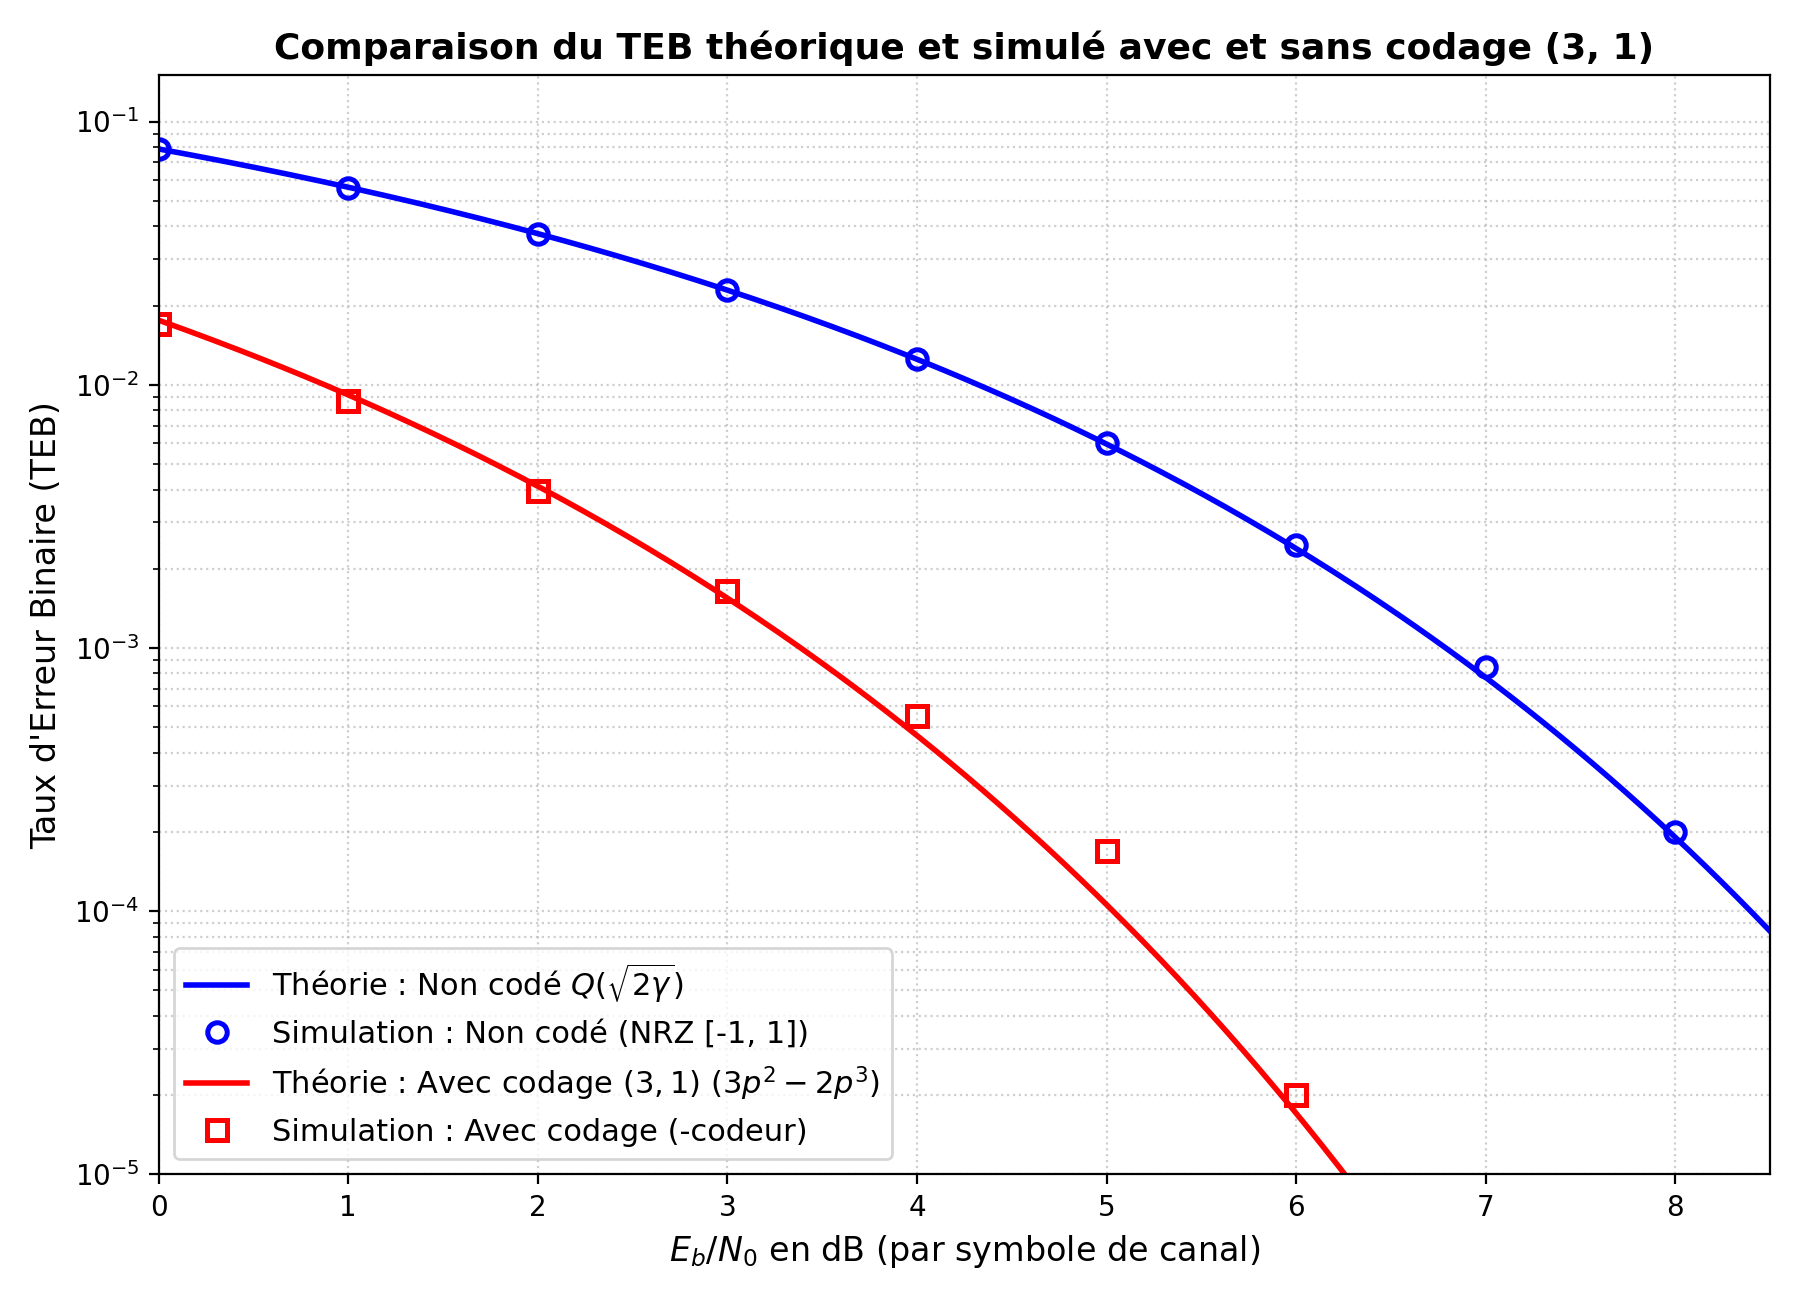
\includegraphics[width=0.75\linewidth]{figures/courbe_teb_codeur.png}
    \caption{Courbes de TEB en fonction de $E_b/N_0$ avec et sans codage de canal. \textit{(Figure à insérer : graphique semi-logarithmique montrant le doublement de la pente et le gain de codage)}}
    \label{fig:courbe_teb_codeur}
\end{figure}

\subsection{Visualisation des signaux à l'aide des sondes}

En invoquant le simulateur avec l'option \texttt{-s}, nous pouvons observer l'état du signal à chaque étape de la chaîne de transmission, comme l'illustre la figure \ref{fig:sondes_tp5}.

\begin{figure}[H]
    \centering
    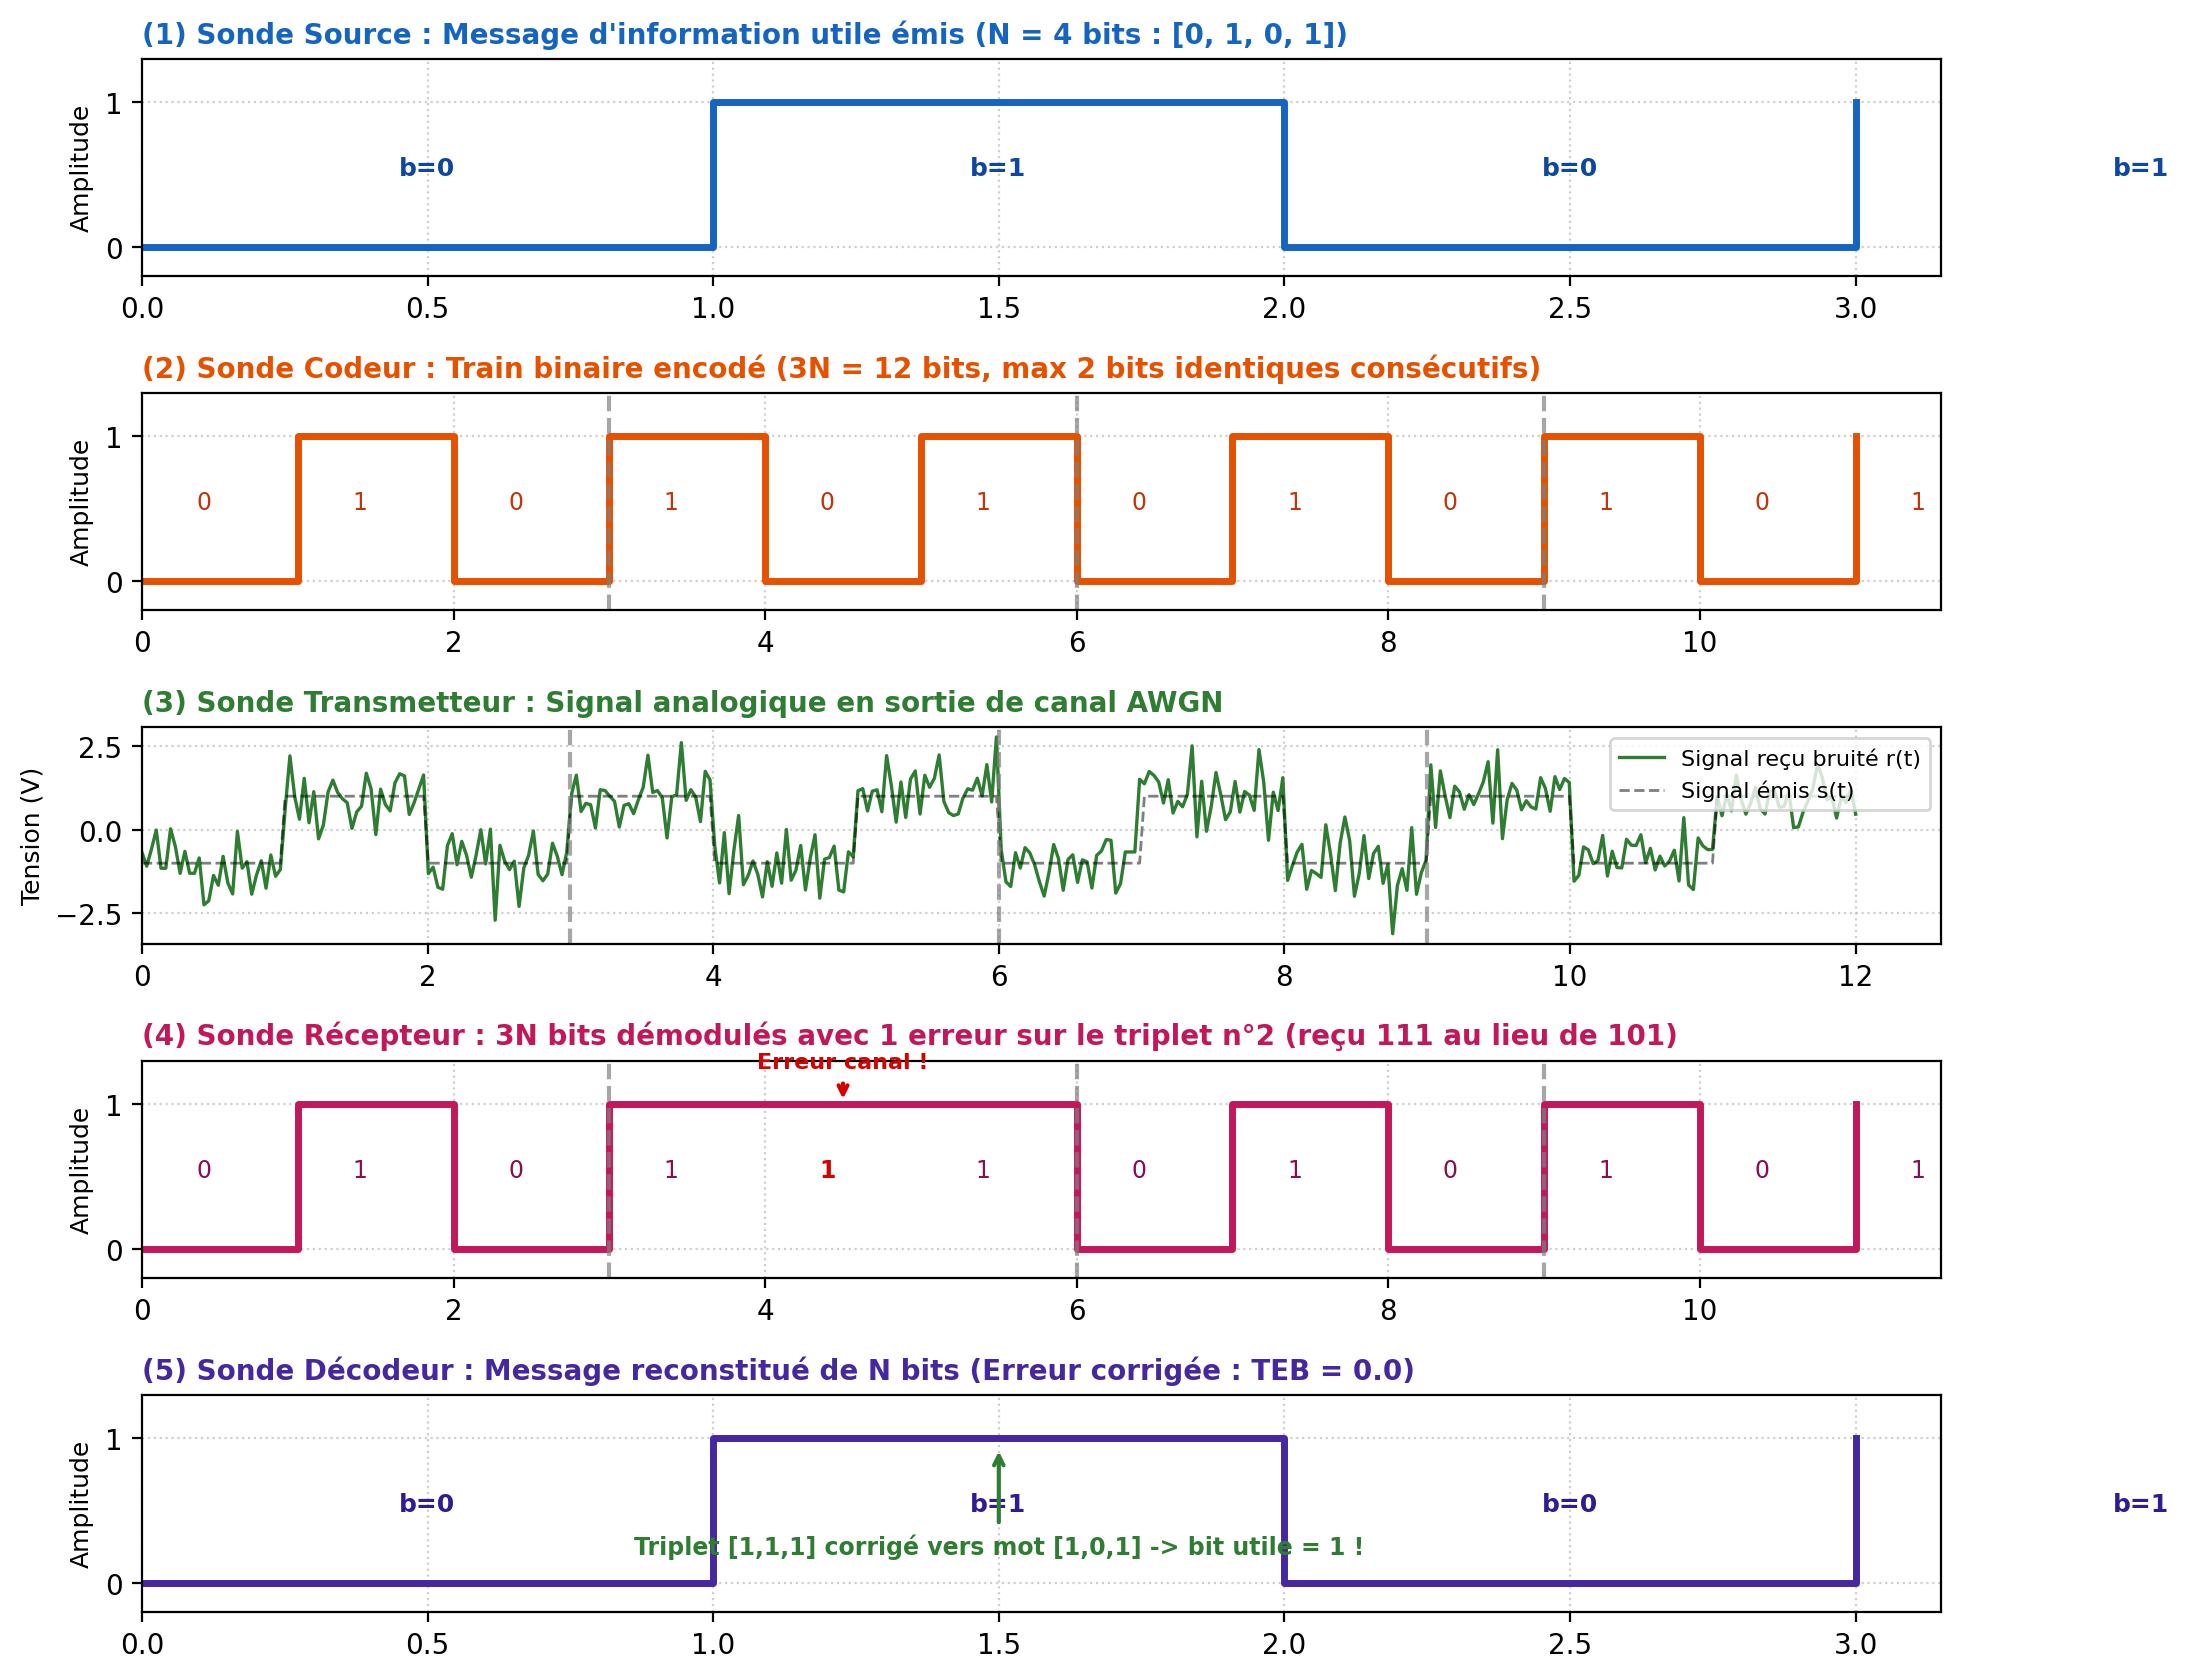
\includegraphics[width=0.9\linewidth]{figures/sondes_tp5.png}
    \caption{Visualisation des sondes logiques et analogiques avec codage de canal. \textit{(Figure à insérer : capture d'écran du simulateur avec commande \texttt{java Simulateur -mess 01010101 -s -form NRZ -snrpb 5 -codeur})}}
    \label{fig:sondes_tp5}
\end{figure}

Les sondes permettent d'observer très distinctement :
\begin{enumerate}
    \item La sonde \textbf{\og{}Source\fg{}} affiche les bits d'origine émis ($N$ bits).
    \item La sonde \textbf{\og{}Codeur\fg{}} affiche le train binaire encodé ($3N$ bits) où l'on remarque l'alternance soutenue et l'absence de répétition de plus de 2 bits identiques.
    \item La sonde \textbf{\og{}Transmetteur\fg{}} montre le signal analogique bruité par le canal AWGN.
    \item La sonde \textbf{\og{}Recepteur\fg{}} montre les $3N$ bits démodulés en sortie de canal, sur lesquels des erreurs isolées apparaissent ponctuellement.
    \item La sonde \textbf{\og{}Decodeur\fg{}} affiche le message de $N$ bits reconstitué : on constate que les erreurs isolées ont été nettoyées par l'algorithme du mot le plus proche, restituant fidèlement le message émis.
\end{enumerate}

\section{Utilisation de l'IA}

Dans la continuité des chapitres précédents, nous avons documenté notre utilisation des modèles de langage dans le fichier \verb|ai_prompts.md|.

Pour cette cinquième itération, nous avons principalement sollicité l'IA dans les domaines suivants :
\begin{itemize}
    \item \textbf{Modélisation théorique :} Nous avons interrogé Gemini pour vérifier l'exactitude de notre dénombrement combinatoire sur le canal BSC ($P_e = 3p^2 - 2p^3$) et confirmer l'équivalence entre la règle du mot le plus proche et le vote majoritaire sur les bits modifiés.
    \item \textbf{Conception logicielle et automates :} L'enseignant suggérant l'utilisation du formalisme des automates, nous avons demandé à Claude de nous proposer une structure de transducteur fini déterministe synchrone en Java pour la méthode \texttt{recevoir()} du décodeur. Nous avons ensuite adapté et épuré ce code pour respecter scrupuleusement la charte de programmation et les conventions du projet.
    \item \textbf{Conception des tests :} Gemini nous a aidé à dresser la liste exhaustive des cas de test pour le décodeur (test individuel des 8 triplets et vérification systématique du bit erroné).
    \item \textbf{Rédaction LaTeX :} Gemini a été utilisé pour nous aider à composer les tableaux de synthèse et vérifier l'orthographe du chapitre.
\end{itemize}

\section{Conclusion}

Cette cinquième et dernière itération finalise notre simulateur de chaîne de transmission numérique avec l'intégration du codage de canal. 

Grâce à un code en bloc $(3, 1)$ à décision par recherche du mot le plus proche, nous avons pu constater une diminution très nette du Taux d'Erreur Binaire en présence de bruit gaussien, passant d'un comportement d'ordre 1 à un comportement d'ordre 2 ($P_{e,\text{codé}} \approx 3p^2$). Nous avons également analysé la propriété de synchronisation du code, tout en justifiant avec rigueur pourquoi notre simulateur à échantillonnage idéal ne permet pas d'en quantifier le gain d'horloge.

L'ensemble des composants respecte les principes de conception orientée objet et de génie logiciel préconisés à IMT Atlantique : séparation des responsabilités, robustesse aux entrées invalides, couverture de tests à 100\% et documentation Javadoc complète.
\thispagestyle{main}

%\listoftables
%\thispagestyle{main}

\printglossary[type=main]
\thispagestyle{main}

\printglossary[type=acronym]
\thispagestyle{main}

%\chapter*{Annexes}
%\thispagestyle{main}

\end{document}